\documentclass[12pt]{report}

% Packages
\usepackage{amsmath}
\usepackage{graphicx}
\graphicspath{{img/}}
\usepackage{setspace}
\usepackage{geometry}
\usepackage{natbib}
\usepackage{tabularx}
\usepackage{array}
\usepackage{hyperref}
\usepackage{microtype}
\usepackage{ragged2e}

\geometry{margin=1in}
\onehalfspacing
\setcounter{tocdepth}{2}
\hypersetup{hidelinks}

\begin{document}
\justifying
	\begin{center}
		{\huge{\textbf{ Mathematical Modelling and Statistical Analysis for Predicting Students’ Academic Performance Using Multivariate Factors }}}
	\end{center}
	
	\begin{center}
		by\\
		\vspace{1.4cm}
		\Large{\bf{EHIME, KELVIN EHINOMEN}}
	\end{center}
	
	\vspace{1.4cm}
	\begin{center}
		Matric Number: 22010303003
	\end{center}
	
	\vspace{3cm}
	\begin{center}
		A PROJECT SUBMITTED TO THE DEPARTMENT OF COMPUTER SCIENCE\\
		AND MATHEMATICS, COLLEGE OF BASIC AND APPLIED SCIENCES,
	\end{center}
	\begin{center}
		IN PARTIAL FULFILLMENT OF THE REQUIREMENTS FOR THE AWARD OF\\
		DEGREE OF BACHELOR OF SCIENCE IN MATHEMATICS.
	\end{center}
	
	\vspace{3cm}
	\begin{center}
		AUGUST 2026
	\end{center}
	
	\newpage
	\begin{center}
		\addcontentsline{toc}{section}{Declaration}
		\Large{\textbf{DECLARATION}}
	\end{center}
	
	\noindent I hereby declare that this project has been written by me and is a record of my own research work. It has not been presented in any previous application for a higher degree of this or any other University. All citations and sources of information are clearly acknowledged by means of reference.
	
	\vspace{1cm}
	\begin{center}
		----------------------------------------------- \\
		\textbf{EHIME, KELVIN EHINOMEN}
	\end{center}
	\begin{center}
		----------------------------------------------- \\
		\textbf{Date}
	\end{center}
	\newpage
	\begin{center}
		\addcontentsline{toc}{section}{Certification}
		\section*{CERTIFICATION}
	\end{center}
	
	\noindent This is to certify that the content of this project entitled ‘\textbf{Mathematical Modelling and Statistical Analysis for Predicting Students’ Academic Performance Using Multivariate Factors}’ was prepared and submitted by \textbf{EHIME, KELVIN EHINOMEN} in partial fulfillment of the requirements for the degree of \textbf{BACHELOR OF SCIENCE IN MATHEMATICS}.\\The original research work was carried out by her under my supervision and is hereby accepted.
	
	\vspace{3cm}
	\begin{center}
		-----------------------------------------------  (Signature and Date)\\
		Mr. E.G. Hunsipe\\
		Supervisor
	\end{center}
	
	\vspace{3cm}
	\begin{center}
		-----------------------------------------------  (Signature and Date)\\
		Dr. A. A. Mebawondu\\
		Ag. Head, Department of Computer Science and Mathematics
	\end{center}
	
	\newpage
	\begin{center}
		\addcontentsline{toc}{section}{Dedication}
		{\Large{\bf DEDICATION}}
	\end{center}
	
	\begin{quote}
		This project work is dedicated to God the Father, God the Son, and The Holy Spirit. In addition, I also want to express my gratitude to my parents for their unwavering financial, emotional, and spiritual support over the years.
	\end{quote}
	
	\newpage
	\thispagestyle{empty}
	\begin{center}
		\addcontentsline{toc}{section}{Acknowledgements}
		{\Large{\bf Acknowledgements}}
	\end{center}
	
	\noindent First and foremost, I express my heartfelt gratitude to God, without whom I could not have achieved this milestone. I am immensely grateful to my family, particularly my parents (Mr. and Mrs. Ehime) for their unwavering love, support, and prayers throughout this journey.
	
	\noindent I extend my deepest appreciation and indebtedness to Dr. Akindele Mebawondu, my capable supervisor, whose invaluable guidance, encouragement, insightful criticism, and direction have been instrumental in the success of this research project.
	
	\noindent I am grateful to the entire staff of the Department of Computer Science and Mathematics, including Mr. Jeremiah Balogun, as well as other lecturers and non-teaching staff, Dr. Obafemi Young, Pastor Olumide Adesina for their continuous support and guidance throughout the course of my programme.
	
	\noindent I would also like to acknowledge and thank my fellow colleagues and friends, namely [insert names] for their camaraderie and support. Special thanks go to [insert name] for her unwavering belief in my abilities and constant encouragement.
	
	\noindent Additionally, I would want to thank and honor everyone who has helped this project be completed successfully in whatever manner. Their assistance has been priceless, and I sincerely appreciate it.

	\newpage
	\begin{center}
		\addcontentsline{toc}{section}{Abstract}
		{\Large{\bf Abstract}}
	\end{center}
	
	\noindent This study develops and evaluates a predictive model for students' academic performance at Mountain Top University using mathematical modelling, ordinary least squares (OLS) regression, and time series analysis on per-level GPA. The primary outcome is Level~400 GPA (CGPA400), predicted from lagged three-year performance (\textit{Previous\_GPA}), prior academic trajectory (\textit{Trajectory\_Slope\_Prior}, OLS slope through CGPA100--300 only), synthesized attendance and study hours, course load, haemoglobin genotype, and a health-pathway interaction for SS students. Registrar data for 3,046 graduates (2010--2014) are enriched with documented synthesis where behavioural and genotype fields were absent from the historical export.
	
	A reproducible Python pipeline (\texttt{enrich.py}, \texttt{verify.py}, \texttt{predict.py}, \texttt{score.py}, \texttt{app.py}) prepares the dataset, runs 52 integrity checks, and reports five-fold cross-validated error on CGPA400 (MAE $= 0.357$, RMSE $= 0.453$, out-of-fold $R^2 = 0.680$; adjusted in-sample $R^2 = 0.682$). Time series components include four-level descriptive trajectory slopes, prior-only slopes used in the scorer, an AR(1) panel on level-to-level GPA transitions ($\hat{\phi}_1 = 0.773$), and a Kendall trend test on cohort mean GPA across Levels 100--400. Results are illustrative under stated synthesis assumptions (L1--L7) and are not presented as causal proof from observed attendance or clinical genotype records.
	
	\vspace{1em}
	\noindent \textbf{Keywords:} Academic performance, CGPA400, Trajectory\_Slope\_Prior, time series analysis, OLS regression, predictive modelling, attendance, study hours, genotype, trajectory classification, AR(1), Mountain Top University, educational data analysis.

	\newpage
	\tableofcontents
	\listoffigures
	\newpage

	\chapter{Introduction}
	
	\section{Background of the Study}
	
	Education is a crucial part of the national development, and one of the most significant metrics applied to evaluate the competence of the educational systems is the academic performance of students. The Grade Point Average (GPA) is usually used to assess academic performance and offer a standardized measure of performance of students over a period. Following the GPA of students on different academic times allows one to identify the trends, consistency and patterns of performance.
	
	The recent years have witnessed an increasing interest in using quantitative methods in educational research. Specifically, Mathematical Modelling has become an effective means of modeling real-world problems in mathematical forms, and Statistical Analysis offers ways of interpreting information and making informed decisions in the uncertain world. By using these methods, researchers are able to go beyond the descriptive analysis and come out with predictive models that have the ability to predict the academic performance of students based on the predictable factors.
	
	The academic, behavioral, and physiological factors interact to affect academic performance. Of these, study habits, usually quantified in the number of average hours of study, are sensitive factors in determining the degree to which students acquire knowledge. Likewise, the attendance at classes has a significant influence since it indicates the level of student participation and exposure to instructional activities and these directly influence the learning outcomes. Moreover, the course load can influence the capability of students to manage time well and be able to perform consistently.
	
	In addition to these academic and behavioral variables, growing awareness is being given to the health related variables in determining the academic performance of students. The biological traits like genotype may affect the overall health status of a person. Indicatively, some genotypes can be linked to health issues, which could result in low attendance, poor concentration or disruption of studies. Consequently, the inclusion of this kind of variables in the academic performance models offers a more realistic and holistic explanation of the learning conditions of students.
	
	Although there are studies on the academic performance of students, a large proportion of the available studies consider individual factors or apply restricted methods of analysis. Not many studies embrace the use of an integrated modelling approach that incorporates various influencing variables in a single framework. This weakness minimizes the capacity to determine the intricate interactions among factors which influence academic performance.
	
	Hence, a more detailed and data-also-driven method of the combination of many determinants of academic performance in a single form of analysis is needed. This paper fills this gap by using mathematical modelling and statistical analysis methodologies to assess and predict academic performance of students using important variables like GPA, studying hours, attendance, and genotype. In this way, the proposed research will bring a better understanding of the dynamics of academic performance and help create forecasting tools that may be applied to the educational planning and intervention approaches.
	
	
	
	\section{Statement of the Problem}
	
	There are numerous aspects that determine the academic performance of students such as studying habits, classroom attendance, and health status. Most of the existing researches, however, are likely to investigate these factors separately and not the cumulative impact of the factors on the overall academic performance of the students. This disjointed methodology restricts a wholesome conception of the interaction of these variables to shape performance.
	
	Moreover, there are no systematic models that can serve efficiently in analyzing and predicting the academic performance of students based on a combination of multiple variables. Most of the conventional ones are based on the descriptive statistics that lack adequate predictive power and understanding of the relations between the major factors of influence.
	
	Moreover, the lack of unified datasets that combine academic, behavioral, and health-related data, including genotype, is a limitation to the creation of effective and trustworthy models. Such a gap prevents educators and institutions to detect at-risk students at an early stage and introduce interventions based on data.
	
	Consequently, a mathematical and statistical model that would combine various determining factors is necessary to effectively study and forecast academic performance of students.
	
	\subsection{Research Gap and Contribution}
	Although there are numerous studies on the academic performance of the students, a number of gaps in the literature still remain. Most of the past researches have been inclined to look at individual factors like study habits or attendance separately, and not in a combination of both. This restricts a thorough examination of the interaction of the various academic, behavioral, and health-related factors to determine how these factors affect the performance of students.
	
	Moreover, majority of the studies that are available do not take into account the contribution of health-related factors like genotype. This exclusion makes the analysis incomplete, particularly where health status can be a major factor influencing academic activity of students, attendance, and their overall performance.
	
	In addition, many of the studies are based on descriptive statistical analysis not predictive modelling techniques. Consequently, these researches are unable to predict academic performance or give practical measures to intervene at the initial stages. The other important limitation is the lack of detailed datasets which capture all the important variables such as GPA in all semesters, hours of studying, attendance, and genotype. This complicates the process of coming up with strong and effective models.
	
	In addition, not all of the existing models are sufficiently tested on independent real-life data, and it is questionable as to how well they would perform in real-life environments and how representative they are.
	
	This research fills these gaps by coming up with an integrated model of prediction, which incorporates a combination of various factors of influence, such as GPA, hours of study, attendance, and genotype. The study offers explanatory and predictive information on the academic performance of students by using the Mathematical Modelling and Statistical Analysis, which is regression analysis.
	
	Moreover, the research presents genotype as an innovative variable, which, in turn, introduces an aspect of health-related approach that is frequently neglected in academic performance research. In order to address the limitations of data, both real-life and simulated data sets are used in the study to achieve completeness of variables but still retain realism.
	
	Lastly, the model developed is tested with independent real-life data, which increases its validity and practicality. The result of the study can be taken as a helpful predictive instrument that may help educators and academic organizations to recognize at-risk pupils and make evidence-based and rational decisions.
	
	\section{Aim and Objectives of the Study}
	This study will focus on coming up with a mathematical and statistical model of analysing and predicting the academic performance of the students using a variety of factors that affect the performance of the students, including the study hours, attendance and genotype in this case.
	
	\begin{itemize}
		\item To analyze students’ academic performance using GPA data across different academic periods.
		\item To examine the relationship between academic performance and key factors such as study hours, attendance, and genotype.
		\item To develop a regression-based mathematical model for predicting students’ academic performance.
		\item To test the developed model on the real-life data and determine its predictive accuracy.
	\end{itemize}
	
	\section{Methodology}
	This study adopts a quantitative research approach to analyze and predict students’ academic performance using Mathematical Modelling and Statistical Analysis. The methodology involves the use of both real-life and simulated datasets to ensure completeness and reliability of the variables considered in the study.
	
	The data utilized include students’ Grade Point Average (GPA) across multiple semesters, average study hours per week, average attendance per semester, and genotype as a health-related factor. Where real-life data are incomplete, simulated data are generated to incorporate missing variables such as genotype, thereby ensuring a comprehensive dataset for analysis.
	
	Prior to analysis, data preprocessing techniques are applied. These include data cleaning, handling missing values, normalization of variables, and proper structuring of the dataset to make it suitable for modelling. The independent variables considered in this study are study hours, attendance, and genotype, while the dependent variable is students’ academic performance measured by GPA.
	
	A multiple regression model is employed to examine the relationship between the dependent and independent variables. The model is mathematically expressed as:
	\subsection{Regression Model Specification}
	
	The multiple regression model used in this study is expressed as:
	
	\begin{equation}
		Y = \beta_0 + \beta_1 X_1 + \beta_2 X_2 + \beta_3 X_3 + \varepsilon
	\end{equation}
	
	This introductory specification captures the three core behavioural
	predictors described in the research objectives. The full empirical
	model fitted in Chapter~3 extends this to seven terms, adding lagged
	academic performance (\textit{Previous\_GPA}), course load, and a
	genotype-attendance interaction term for SS students.
	
	\subsection*{Where:}
	
	\begin{itemize}
		\item $Y$ = Students’ academic performance (measured by GPA)
		\item $X_1$ = Average study hours
		\item $X_2$ = Average attendance
		\item $X_3$ = Genotype
		\item $\beta_0$ = Intercept (constant term)
		\item $\beta_1, \beta_2, \beta_3$ = Regression coefficients
		\item $\varepsilon$ = Error term
	\end{itemize}
	
	This model shows that students’ academic performance depends on study hours, attendance, and genotype, while the error term captures other influencing factors not included in the model.
	
	\section{Significance of the Study}
	This study is important since it is a contribution to the use of Mathematical Modelling and Statistical Analysis in the solution of educational problems on students academic performance. The study establishes a regression model prediction system that provides a systematic solution for analyzing the relationship between academic performance and factors affecting it (study hours, attendance, genotype).
	The study is useful for students, teachers, researchers and institutions. As a study for students, the study aims to identify the factors that affect the success of a student's study and at the same time encourage students to improve their study habits and class participation. Developed model can be used as a decision support tool for educators/institutions to monitor students' progress and determine students who need academic intervention.
	In addition, this study is an addition to the current literature that also combines academic, behavioral, and health variables in one analysis. Incorporating genotype adds another layer of consideration that's missing from studies around educational performance.
	The study also illustrates the use of regression analysis and prediction modelling methods using computational software like Python or MATLAB. This reflects the trend in educational research and decision making to increasingly make use of information.
	Lastly, the results and procedures of the present work could be used as a reference for future researchers related to academic performance prediction, education data analysis, and applied mathematical modelling.
	\section{Overview of Methodology}
	The methodology of this study is quantitative and prediction type research with Mathematical Modelling and Statistical Analysis techniques used to analyze and predict student academic performance. The methodology consists of gathering academic-related data from students such as GPA during each semester, semester attendance, number of courses taken, study hours and genotype.
	
	The gathered information is then processed to standardize its consistency and applicability for analysis, including steps like cleaning, organizing, encoding, and normalizing. Then a multiple linear regression model is developed to find the relationship between students' academic performance and selected independent variables.
	
	This regression model is executed with computational tools based on Python and trained with the simulated data and real life data. The model is then tested on other real-world data to assess its predictive power and reliability.
	
	At the end, statistical evaluation measures and graphical representations are used to analyse the performance of the model and to explain the relations between the variables taken into consideration in the study.
	
	\section{Organisation Of Study}
	The research work is divided into five chapters for systematic and logical presentation of the study.
	
	Chapter One contains the general introduction to the study where the background of the study, statement of the problem, aim and objectives of the study, significance of the study, scope of the study, overview of the methodology and organization of the study is presented.
	
	The literature review and theoretical framework are discussed in Chapter Two. It provides a summary of relevant literature in the field of academic performance, study habits, attendance, genotype, regression analysis and predictive modelling methods of students. The chapter also includes discussion of the mathematical and statistical concepts that are important for the study and also the gaps identified in the existing research.
	
	The methodology used in the study is discussed in Chapter Three. It will present to you the research design, data collection methods, dataset preparation and pre-processing techniques, formulation of the regression model and implementation of the model using Python or MATLAB and model validation techniques utilized during the development of the predictive model.
	
	The results of implementing the model, statistical analysis, regression results, graphical visualization, and interpretation of results obtained from the developed predictive model are presented in Chapter Four.
	
	Lastly, Chapter Five concludes the study, summarizes the findings, highlights the limitation of the study and gives recommendations for future research and possible improvements of the developed model.
	
	\chapter{Literature Review and Mathematical Foundations}
	\section{Introduction}
	Several studies have investigated the factors influencing students’ academic performance using statistical and predictive approaches. This section systematically compares selected studies related to study habits, attendance, and predictive modelling techniques in education.
	
	One of the major areas of agreement among existing studies is that academic performance is influenced by measurable behavioral and environmental factors. \citet{Crede2008} concluded that study habits, motivation, and time management significantly contribute to academic success. Similarly, \citet{Stine2008} found that increased study hours positively affect students' academic outcomes. In the same manner, \citet{Romer1993} and \citet{Marburger2006} agreed that class attendance plays a significant role in improving students' GPA and overall academic achievement.
	
	Another point of consensus among these studies is the importance of quantitative analysis in educational research. Most of the reviewed studies employed statistical techniques such as descriptive statistics, correlation analysis, and regression models to establish relationships between academic performance and influencing variables. This demonstrates the growing relevance of Statistical Analysis in educational performance evaluation.
	
	Despite these similarities, some direct debates and conflicting findings exist in the literature. While \citet{Stine2008} argued that study hours have a strong causal relationship with academic performance, other studies suggest that study time alone is insufficient for accurately predicting students' outcomes. Some researchers emphasize that attendance, motivation, learning environment, and psychological factors may jointly influence performance rather than acting independently. This creates debate regarding the most significant predictors of academic achievement.
	
	Similarly, studies on attendance present varying conclusions regarding the magnitude of its impact. \citet{Romer1993} reported a strong relationship between attendance and academic success, whereas some later studies found that attendance alone may not guarantee high performance if effective study habits are absent. These conflicting findings suggest that academic performance is multidimensional and cannot be explained adequately using a single variable.
	
	The methodological approaches adopted by these studies may explain many of the observed differences. Some studies rely primarily on descriptive statistics and correlation analysis, while others employ advanced predictive methods such as regression analysis and educational data mining. Studies using simple descriptive methods often provide general observations but lack predictive capability. In contrast, regression-based studies establish stronger mathematical relationships between variables and provide forecasting ability.
	
	Another methodological difference lies in the datasets used by researchers. Several studies depend on small or institution-specific datasets, limiting the generalizability of their findings. Others rely on self-reported study hours and attendance records, which may introduce measurement bias. Furthermore, most existing studies exclude health-related variables such as genotype, thereby overlooking potential biological influences on academic performance.
	
	Regression analysis remains one of the most widely adopted approaches in educational predictive modelling because it allows multiple variables to be analyzed simultaneously. The general multiple regression equation used in educational prediction studies is expressed as:
	
	\[
	Y = \beta_0 + \beta_1 X_1 + \beta_2 X_2 + \cdots + \beta_n X_n + \varepsilon
	\]
	
	Where:
	
	\begin{align*}
		Y & = \text{Academic performance} \\
		X_1, X_2, \ldots, X_n & = \text{Independent variables such as study hours and attendance} \\
		\beta_0 & = \text{Intercept} \\
		\beta_1, \beta_2, \ldots, \beta_n & = \text{Regression coefficients} \\
		\varepsilon & = \text{Error term}
	\end{align*}
	
	The reviewed studies collectively demonstrate that academic performance prediction requires a multidimensional and integrated modelling approach. However, there remains a gap in combining academic, behavioral, and health-related variables within a single predictive framework. This study addresses that limitation by integrating GPA, study hours, attendance, and genotype into a regression-based predictive model validated using real-life data.
	\section{Academic Performance Assessment}
	Academic performance is the measure of students' success in their learning experiences and evaluations. Usually it is determined by the Grade Point Average (GPA), examination performance and overall record of academic achievement. Student academic achievement is frequently considered as evidence of their learning, engagement and persistence in learning activities.
	
	In addition to intelligence, academic performance depends on behavior and environment factors like time management, class participation and study habits \citep{Crede2008}. Their research highlighted the importance of cognitive and non-cognitive factors contributing to academic achievement.
	
	Academic performance analysis is a crucial tool for educational institutions that aims to assess the effectiveness of the curriculum, the quality of teaching, and the engagement of students. Academic analysis that is accurate enables the institutions to identify students in need of academic support and helps teachers to come up with intervention measures.
	
	While academic performance evaluation is always of great importance, traditional methods of academic performance evaluation are usually using descriptive methods which are not capable of capturing the complex relationships between influencing variables. This restriction has led to the use of techniques that have come into use in the field of educational research, such as predictive modelling and statistical analysis.
	\section{Study Hours and Academic Performance}	
	Factors that are likely studied that affect academic achievement include study habits and study duration. Study hours are time spent by students in studying activities outside of the regular class time. Good Study Skills promote knowledge, understanding and examination performance.
	
	\citet{Stine2008} studied the link between study time and academic achievement and decided that prolonged academic study time positively affects students' academic results. They found that pupils who put in regular and significant time into their studies are more likely to get better academic outcomes.
	
	Likewise, \citet{Crede2008} found that good study skills were significantly linked to increased GPAs and academic stability.
	
	Several studies do highlight, however, that study time is not the only factor to consider when determining academic achievement; attendance, motivation, health and environment also play a role. This implies the need for a combination of multiple variables and for integrated models as opposed to models involving only one variable as their sole focus.
	\section{Attendance and Academic Performance}
	Attendance is a reflection of student involvement and participation in school activities. Good attendance ensures that students have access to lecture, discussion, practical and interaction that improves their learning outcomes.
	
	\citet{Romer1993} studied the connection between school attendance and academic performance, and he found that students who are on a regular attendance schedule do better than those who have poor attendance records. Likewise, \citet{Marburger2006} discovered that students' academic achievement is enhanced by required attendance.
	
	Attendance is a key factor in academic achievement, enhancing learners' access to learning materials and minimizing learning gaps. Frequent absences can cause students to fall behind in their coursework and therefore will not perform as well in the class.
	
	While there has been demonstrated evidence that it is a positive factor in children's academic achievement, many studies only examine attendance, and not encompass other factors like study habits or health-related issues. This will result in a partial report of students' learning.
	\section{Health and Academic Performance}
	Students' productivity, concentration and engagement in school learning is significantly influenced by their health conditions. Illness may impact on attendance, regularity in studies, and the effectiveness of learning.
	
	Genotype is one factor of health that is important to this study. Genotype is the genotype of an individual, which is usually represented as AA, AS or SS. There are health issues that could impair students' ability to participate in educational activities for students with some genotype conditions, especially sickle cell-related conditions.
	
	\citet{WHO2020} stated that sickle cell diseases have negative impact on health status which can impact productivity, attendance and day-to-day functioning. These may have indirect effects on learning.
	
	Although there may be a linkage between genotype and academic achievement, many studies on education do not incorporate health-related factors in prediction models. Existing studies are mainly limited to academic and behavioral factors, leaving out other variables, and this represents a gap in the literature.
	
	Considering the genotype aspect in this study brings new and more complex dimension to academic performance analysis.
	\section{Mathematical Modelling}
	Mathematical modelling is the act of using mathematical models to represent real-world systems and relationships in terms of mathematical expressions and equations. Models are used by researchers to help them simplify complex systems, to analyze the relationship between variables and to predict.
	
	Mathematical models are employed in educational research to investigate students' performance, learning behaviors, and effectiveness of the educational institution. Mathematical models are a systematic way to explain the relationship between various variables and academic outcomes.
	
	In this research, the use of mathematical modelling enables academic achievement to be represented by a function of various influencing variables including study hours, attendance and genotype. This will allow predictive models to be developed which can estimate students' future academic performance.
	
	The transformational value of mathematical modelling is especially pronounced, as it allows the education data to be measurable and interpretable, thus facilitating data-driven decisions.
	\section{Statistical Analysis in Educational Research}
	The analysis of data is called statistical analysis and is concerned with collecting, organising, interpreting and presenting the data. In education research, statistics have been commonly employed for analyzing students' performance, detecting trends, and determining the relationship among the variables.
	
	Descriptive statistics, correlation analysis, hypothesis testing, and regression analysis are common data analysis techniques employed in educational research. Descriptive statistics include measures of central tendency (mean, median, and standard deviation) and correlation analysis measures the strength of relationships between variables.
	
	Through the use of statistical analysis, researchers are able to transcend observation and make evidence-based decisions about academic performance. Use of statistical methods also enhances reliability and validity of research findings.
	
	The statistical analysis in this study offers a quantitative approach to analyzing the impact of the selected variables on academic performance.
	
	\section{Regression Analysis}
	Regression analysis is a statistical technique used to examine relationships between dependent and independent variables. It is widely used for prediction and forecasting in various fields, including education, economics, engineering, and health sciences.
	
	According to \citet{Montgomery2012}, regression analysis provides a mathematical framework for estimating the effect of multiple variables on a specific outcome.
	
	The regression model used in this study is represented as:
	
	\[
	Y = \beta_0 + \beta_1 X_1 + \beta_2 X_2 + \beta_3 X_3 + \varepsilon
	\]
	
	This general form is consistent with the specification adopted across
	the reviewed literature. The empirical implementation in Chapter~3
	extends it with two additional constructs grounded in the available
	registrar data: lagged cumulative GPA (\textit{Previous\_GPA}) and
	\textit{Course\_Load}, plus a health-pathway interaction for
	haemoglobin genotype SS students.
	
	Where:
	
	\begin{align*}
		Y & = \text{Students' academic performance (GPA)} \\
		X_1 & = \text{Study hours} \\
		X_2 & = \text{Attendance} \\
		X_3 & = \text{Genotype} \\
		\beta_0 & = \text{Intercept} \\
		\beta_1, \beta_2, \beta_3 & = \text{Regression coefficients} \\
		\varepsilon & = \text{Error term}
	\end{align*}
	
	Regression analysis is suitable for this study because it allows multiple factors to be analyzed simultaneously while also providing predictive capability.
	
	\section{Predictive Modelling in Education}
	Predictive modelling is the process of using statistical or computational methods to predict future outcomes based on past data. The key value in using educational predictive models is their ability to predict students' academic outcomes, to assist in identifying students who may be at risk, and to help institutions plan more effectively.
	
	\citet{Romero2010} have pointed out the increasing significance of the learning data mining and predictive analysis in learning systems. Likewise, \citet{Shahiri2015} stated that predictive models can enhance the monitoring and intervention processes in the academic field.
	
	Predictive modelling is used to identify students who are at risk of academic difficulties early. This allows institutions to take corrective action in good time before the performance starts to suffer.
	
	\section{Research Gap}
	Despite the numerous studies conducted on students’ academic performance, several important gaps still exist in the literature. Most previous studies focus on individual factors such as study habits, attendance, or socio-economic background independently, without integrating multiple influencing variables into a unified analytical framework. As a result, many existing models fail to provide a comprehensive understanding of the combined effects of academic, behavioral, and health-related factors on students’ performance.
	In addition, many studies rely primarily on descriptive statistical methods and correlation analysis, which explain relationships between variables but offer limited predictive capability. Although some researchers have applied regression analysis and predictive modelling techniques, many of these models are developed using limited datasets and are not adequately validated using independent real-life data. This reduces their reliability and practical applicability in real educational environments.
	Another major gap identified in the literature is the exclusion of health-related variables such as genotype. Existing studies rarely consider biological or health conditions that may influence students’ attendance, concentration, productivity, and overall academic engagement. Consequently, current predictive models may not fully capture important factors affecting students’ academic performance.
	Furthermore, many educational performance studies utilize datasets that are incomplete or institution-specific, thereby limiting the generalizability of their findings. The absence of integrated datasets containing academic, behavioral, and health-related variables creates challenges in developing robust predictive systems.
	Therefore, this study seeks to address these gaps by developing a regression-based predictive model that integrates multiple variables, including GPA, study hours, attendance, and genotype. The study also combines simulated and real-life datasets and validates the developed model using independent real-world data to improve reliability, accuracy, and practical relevance.
	
	The fitted empirical model (Chapter~3) therefore uses observed cumulative and per-level GPA from institutional records, statistically synthesized behavioural and health-related fields where records were incomplete, and ordinary least squares (OLS) with out-of-sample validation rather than a machine-learning train--test partition.
	
	\section{Theoretical Framework}
	The theory used for this study is regression analysis and predictive modelling because it is a systematic approach in statistics applied to analyze the relationship between the dependent variable and an independent variable or more than one independent variable. The theory of regression is frequently used in the educational research due to its ability to determine, measure and predict the influence of various factors on academic performance.
	
	This study has a theoretical assumption that the achievement in student learning is not just by chance but is significantly influenced by the measurable variables such as genotype, student attendance and student study time. These are deemed to be important predictors as they are related to academic behaviour, level of engagement in learning activities and biological characteristics that might indirectly impact learning capacity and performance.
	
	The framework is based on the functional relationship between the dependent variable (Grade Point Average (GPA) of the students) and the selected independent variables, modeled using a multiple regression model. In this relationship, GPA is the dependent variable, and study hours, attendance and genotype are independent variables for which variations in students' academic achievement can be explained.
	
	The study also assumes that the changes in the independent variables could result in changes in academic performance. For example, more study time and class attendance should have a positive impact on student's GPA, and genotype might be affected by different health and physiological factors. These relationships can be statistically measured with respect to their strength, direction and significance by regression analysis.
	
	Secondly, predictive modelling can be used to predict students' future academic performance with existing information. This will enable the study to not only capture relationships among the variables, but also to forecast academic performance based on the observed relationships. The model's predictive ability improves the decision-making process for teaching and learning planning and evaluation.
	
	Thus, the framework offers the mathematical and statistical underpinning for understanding the relationships between variables, for testing of hypotheses, and for the generation of predictive models that can accurately and reliably estimate students' academic outcomes with a reasonable level of accuracy.
	
	\chapter{Methodology: Design and Implementation}
	
	\section{Introduction}
	This chapter describes the research design, data sources, variable construction, regression specification, estimation procedures, and predictive validation used to analyse and forecast students' academic performance at Mountain Top University (MTU). The workflow is fully reproducible: enrichment (\texttt{enrich.py}), automated integrity checks (\texttt{verify.py}), exploratory and inferential analysis (\texttt{model.ipynb}), out-of-sample evaluation (\texttt{predict.py}), and operational scoring for new cases (\texttt{score.py}).
	
	\section{Research Design}
	The study adopts a quantitative, explanatory and predictive design. Explanatory analysis estimates the linear association between Level~400 GPA (CGPA400) and selected academic, behavioural, and health-related predictors using multiple OLS regression with standard diagnostic tests. Predictive analysis reports k-fold out-of-sample error (mean absolute error, root mean squared error, and stacked out-of-fold $R^2$) and provides a scoring interface for hypothetical student profiles. All synthesis uses a fixed random seed (42) so results can be replicated exactly.
	
	\section{Study Setting and Data Sources}
	Secondary data comprise 3,046 graduate records from MTU spanning 17 programme codes and graduation years 2010--2014. The immutable source file is \texttt{academic\_performance\_dataset\_V2.csv}. Table~\ref{tab:data-sources} classifies variables by origin.
	
	\begin{table}[htbp]
		\centering
		\caption{Classification of variables in the enriched dataset}
		\label{tab:data-sources}
		\small
		\begin{tabularx}{\textwidth}{@{}>{\raggedright\arraybackslash}p{2.4cm} >{\raggedright\arraybackslash}p{4.6cm} >{\raggedright\arraybackslash}X@{}}
			\hline
			\textbf{Class} & \textbf{Variables} & \textbf{Notes} \\
			\hline
			Observed & ID, programme, gender, YoG, CGPA, CGPA100--400, SGPA & From registrar records; no missing values. \\
			Derived & Previous\_GPA & Mean of CGPA100, CGPA200, CGPA300 (lagged three-year average). \\
			Synthesized & Attendance\_Rate, Study\_Hours\_Per\_Week, Course\_Load, Genotype & Not in source export; generated in \texttt{enrich.py}. \\
			Derived (trajectory) & Trajectory\_Slope\_Prior, Trajectory\_Class\_Prior & OLS slope across CGPA100--300 only; used in OLS/scorer (no CGPA400 leakage). \\
			Derived (descriptive) & Trajectory\_Slope, Trajectory\_Class & Four-level slope across CGPA100--400; EDA and time-series tab only. \\
			\hline
		\end{tabularx}
	\end{table}
	
	Attendance, weekly study hours, course load, and haemoglobin genotype were absent from the historical export and could not be recovered retrospectively. They were synthesized under documented assumptions (Sections~\ref{sec:synthesis}--\ref{sec:genotype-synth}). CGPA and per-level GPAs are treated as observed administrative outcomes on MTU's 0--5 scale.
	
	\section{Data Preprocessing}
	Preprocessing steps were: (i)~load the raw CSV without modification; (ii)~derive \textit{Previous\_GPA} and trajectory columns; (iii)~synthesize missing predictors (genotype before attendance, with genotype-conditioned attendance shifts); (iv)~run 52 automated checks in \texttt{verify.py} (exit code 0 required before modelling); (v)~for analysis notebooks and apps, drop duplicate \textit{ID No} rows where programme, gender, or graduation year conflict (70 collision IDs in the source---data-entry errors, not enrichment artefacts), retaining the first occurrence ($n = 2{,}974$ students for regression).
	
	No imputation of nulls was required in the source file. Variables were not normalized for OLS estimation; coefficients are reported on the original scales (percentage attendance, hours per week, integer course count, and genotype indicators).
	
	\section{Variable Operationalization}
	\label{sec:operationalization}
	\textbf{Dependent variable:} CGPA400, the student's Level~400 (final-year) grade point average on the 0--5 scale. This removes arithmetic overlap with \textit{Previous\_GPA}, which uses only CGPA100--300.
	
	\textbf{Previous\_GPA:} $\text{Previous\_GPA} = (\text{CGPA100} + \text{CGPA200} + \text{CGPA300})/3$, rounded to four decimal places. This is the mean performance over the first three academic levels and is temporally prior to CGPA400.
	
	\textbf{Trajectory\_Slope\_Prior:} OLS slope of CGPA100--300 against $t = 1, 2, 3$ (GPA points per level). Used in Equation~(\ref{eq:full-model}) and the Streamlit scorer. The four-level \textit{Trajectory\_Slope} (including CGPA400) is retained for descriptive trajectory charts but is \textit{not} used to predict CGPA400, because it would leak the outcome.
	
	\textbf{Course\_Load:} Number of courses registered per semester (integer, range 8--20), programme-stratified; not credit units.
	
	\textbf{Attendance\_Rate} and \textbf{Study\_Hours\_Per\_Week:} Synthesized behavioural measures (Sections~\ref{sec:synthesis}).
	
	\textbf{Genotype:} Categorical haemoglobin genotype AA, AS, or SS (Section~\ref{sec:genotype-synth}).
	
	\section{Synthesis of Behavioural Variables}
	\label{sec:synthesis}
	To mitigate endogeneity, attendance and study hours use a \textit{blended} generative model with blend parameter $\alpha = 0.60$:
	\begin{equation}
		X = \alpha \cdot X_{\text{base}} + (1 - \alpha) \cdot X_{\text{corr}} + \eta,
	\end{equation}
	where $X_{\text{base}}$ is drawn from a CGPA-independent population distribution, $X_{\text{corr}}$ is a linear function of CGPA, and $\eta$ is Gaussian noise. Values are clipped to plausible ranges (attendance 40--100\%; study hours 2--20 per week). At $\alpha = 0.60$, Pearson correlations with CGPA are approximately 0.28 (attendance) and 0.24 (study hours), reflecting weak but non-zero behavioural association rather than near-deterministic reconstruction of CGPA.
	
	Course load is drawn from programme-specific truncated normal distributions (e.g.\ CIS/MIS heavier than MAT), with about 5\% of students assigned an approved overload (16--20 courses). Course load is structurally independent of CGPA ($|r| \approx 0.03$).
	
	\section{Synthesis of Genotype}
	\label{sec:genotype-synth}
	Genotype is assigned by a multinomial draw with probabilities $P(\text{AA}) = 0.75$, $P(\text{AS}) = 0.24$, $P(\text{SS}) = 0.01$, reflecting illustrative Nigerian population priors. The draw is \textit{not} taken from student health records. Genotype is synthesized \textit{before} attendance: AS students receive a $-2.5\%$ mean attendance shift and SS students $-8\%$ relative to AA (health-pathway assumption). In regression, AA is the reference category; AS and SS enter as dummies, with an interaction \texttt{Genotype\_SS} $\times$ \textit{Attendance\_Rate} allowing the attendance slope for SS students to differ from AA.
	
	\section{Regression Model Specification}
	The empirical multiple linear regression model is:
	\begin{equation}
		\begin{split}
			\text{CGPA400}_i ={} & \beta_0 + \beta_1 \text{Previous\_GPA}_i
				+ \beta_2 \text{Trajectory\_Prior}_i
				+ \beta_3 \text{Attendance}_i + \beta_4 \text{StudyHours}_i \\
			& + \beta_5 \text{CourseLoad}_i + \beta_6 D_{\text{AS},i}
				+ \beta_7 D_{\text{SS},i} \\
			& + \beta_8 \bigl(D_{\text{SS},i} \times \text{Attendance}_i\bigr)
				+ \varepsilon_i,
		\end{split}
		\label{eq:full-model}
	\end{equation}
	where $\text{Trajectory\_Prior}_i$ is the OLS slope through CGPA100--300 for student $i$, and $D_{\text{AS}}$, $D_{\text{SS}}$ are genotype indicators (reference: AA). Equation~(\ref{eq:full-model}) extends the three-predictor specification in Chapter~1 with lagged level, prior trajectory, course load, and a health-pathway interaction for SS students.
	
	OLS assumptions (linearity, independent errors, homoskedasticity, and approximate normality of residuals) were assessed graphically via residuals-versus-fitted, Q--Q, and scale-location plots (Chapter~4). VIF for continuous predictors and \texttt{Genotype\_AS} were below 10; VIF for \texttt{Genotype\_SS} and the SS$\times$attendance interaction are inflated by construction (collinear block) and are reported separately.
	
	\section{Estimation and Diagnostic Procedures}
	Models were estimated with \texttt{statsmodels} OLS on the deduplicated enriched dataset. Reported inferential quantities include coefficient estimates, standard errors, $t$-statistics, $p$-values, and 95\% confidence intervals. Adjusted $R^2$ is reported alongside raw $R^2$. Coefficients on synthesized behavioural variables and genotype are interpreted as illustrative associations under the generative assumptions, not as causal effects (Limitations L1, L3, and L7 in Section~\ref{sec:limitations-results}).
	
	\section{Predictive Validation and Scoring}
	Out-of-sample performance was evaluated with $k$-fold cross-validation ($k = 5$, random seed 42): within each fold, OLS was fitted on the training partition and used to predict CGPA400 on the held-out partition; errors were stacked across folds. Reported metrics are mean absolute error (MAE), root mean squared error (RMSE), and out-of-fold $R^2$, compared to a baseline that always predicts the training-fold mean CGPA400. This is described as \textit{model fitting and out-of-sample validation}, not as a separate machine-learning training and testing pipeline.
	
	For operational forecasts, the same specification was refit on all deduplicated training rows; new input rows (CSV or JSON) supply attendance, study hours, course load, genotype, and either \textit{Previous\_GPA} or CGPA100--300 (from which \textit{Previous\_GPA} and \textit{Trajectory\_Slope\_Prior} are computed). The Streamlit scorer reports a per-term prediction breakdown. Rows with only \textit{Previous\_GPA} and no level GPAs set prior slope to zero (trend not applied). Arbitrary semester-level SGPA sequences without level CGPAs are outside the scope of this model.
	
	\section{Software and Reproducibility}
	Implementation used Python~3.9+ with \texttt{pandas}, \texttt{numpy}, \texttt{scipy}, \texttt{statsmodels} (primary estimation), \texttt{scikit-learn} (cross-validation splits and error metrics), \texttt{matplotlib}, \texttt{seaborn}, \texttt{plotly}, and \texttt{streamlit}. The Streamlit dashboard (\texttt{streamlit run app.py}) reproduces the exploratory, regression, trajectory, and cross-validation views shown in Chapter~4 and Appendix~A. Canonical commands: \texttt{python enrich.py}; \texttt{python verify.py}; \texttt{python predict.py}; \texttt{python score.py}; \texttt{jupyter notebook model.ipynb}; \texttt{streamlit run app.py}.
	
	\section{Methodological Limitations}
	\label{sec:method-limitations}
	Seven limitations govern interpretation: (L1)~residual endogeneity in blended behavioural synthesis; (L2)~overall CGPA still overlaps \textit{Previous\_GPA} if used as DV (primary analysis uses CGPA400); (L3)~synthesized behavioural variables are not observed; (L4)~overload rate and course ceiling assumptions; (L5)~ID collisions in source data; (L6)~parameters calibrated for MTU/Nigeria; (L7)~synthesized genotype and health-pathway attendance shifts, not clinical records. These are discussed again with results in Chapter~4.
	
	\chapter{Results and Analysis}
	
	\section{Introduction}
	This chapter presents descriptive statistics, correlation structure, OLS estimates, regression diagnostics, out-of-sample predictive metrics, and time-series views of per-level GPA. All numerical results below were produced from \texttt{academic\_performance\_enriched.csv} after ID de-duplication ($n = 2{,}974$) with the pipeline described in Chapter~3.
	
	\section{Data Presentation}
	Table~\ref{tab:descriptive} summarizes key numeric variables. CGPA averages 3.50 (SD 0.69) on the 0--5 scale. Synthesized genotype counts were AA = 2,265 (74.4\%), AS = 742 (24.4\%), and SS = 39 (1.3\%), consistent with the multinomial priors ($P(\text{AA})=0.75$, $P(\text{AS})=0.24$, $P(\text{SS})=0.01$). The deduplicated modelling sample ($n = 2{,}974$) contains AA = 2,214, AS = 723, and SS = 37 students. Students span 17 programmes and graduation years 2010--2014.
	
	Figure~\ref{fig:data-overview} shows the Streamlit \emph{Data Overview} tab: the same cohort scope, descriptive statistics for observed and synthesized fields, and genotype counts after ID de-duplication. This establishes who enters the regression and time-series analyses before any modelling assumptions are applied.
	
	\begin{figure}[htbp]
		\centering
		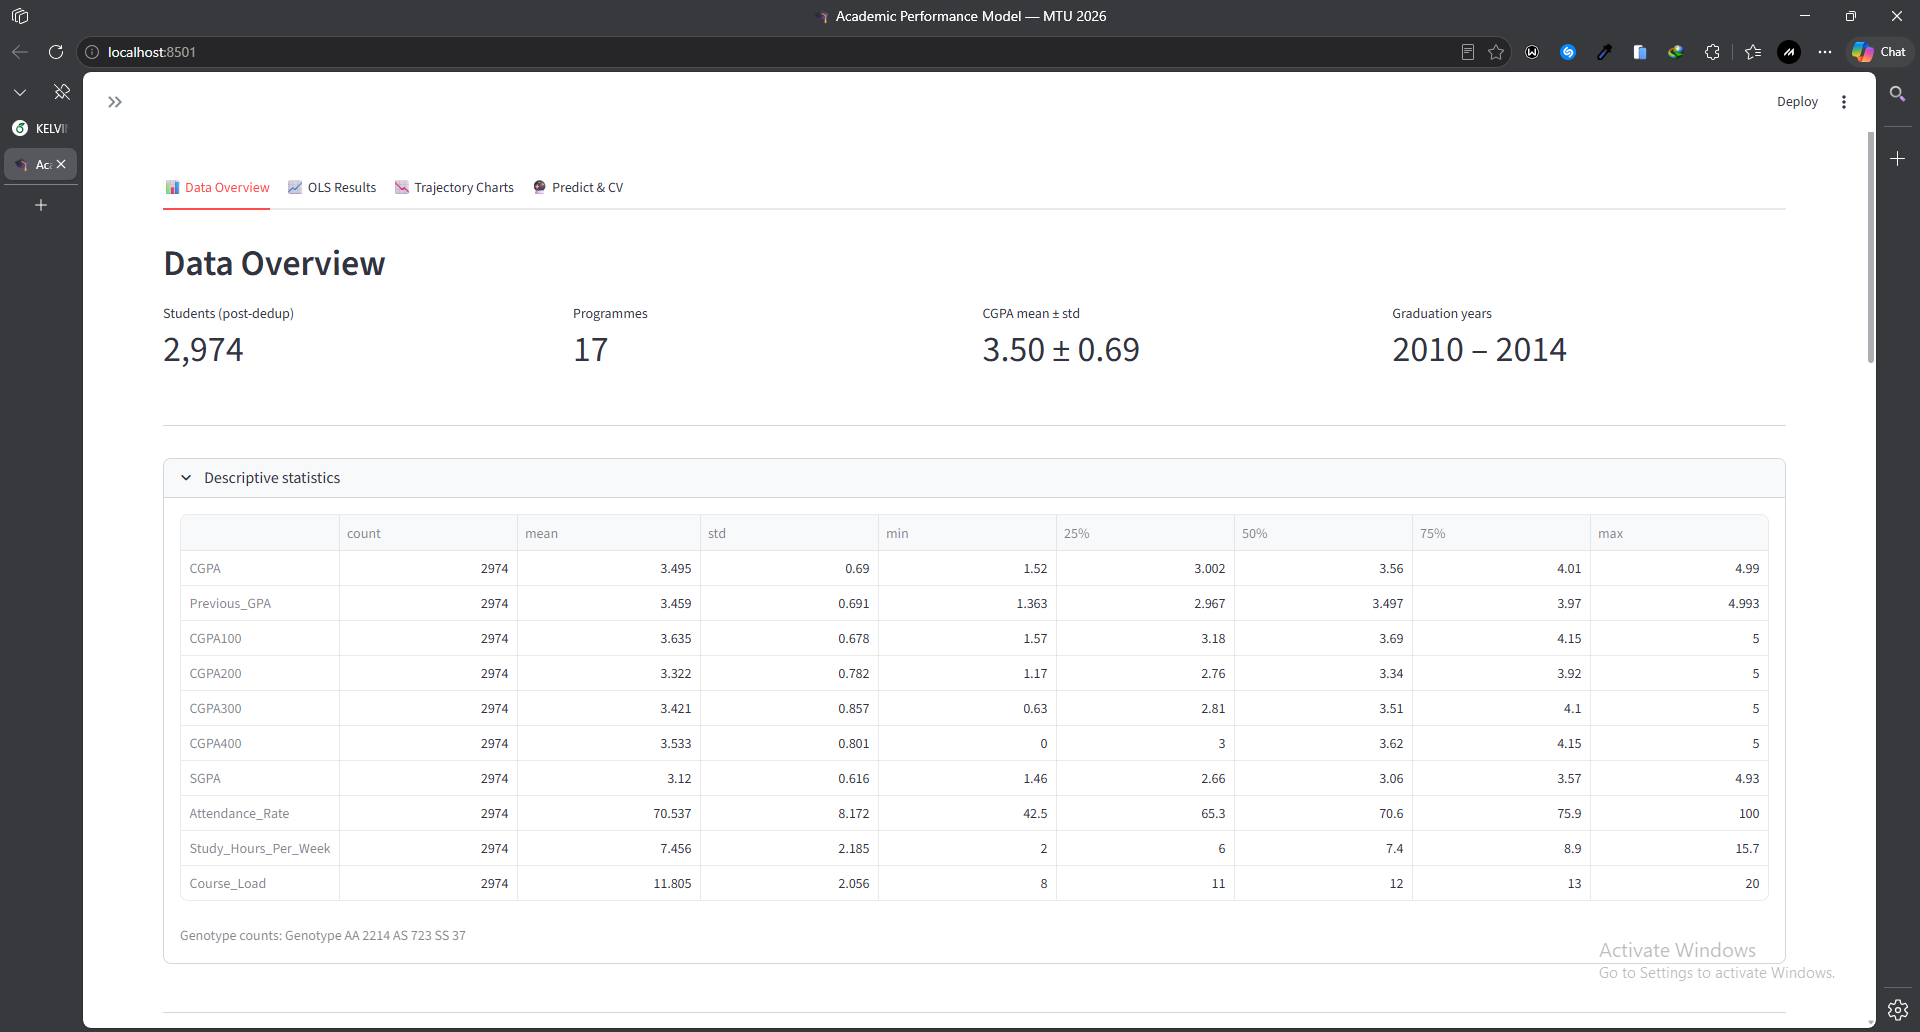
\includegraphics[width=0.92\textwidth]{fig-4-1-data-overview.png}
		\caption{Data overview dashboard ($n = 2{,}974$ after de-duplication; 17 programmes; graduation years 2010--2014). Genotype counts in the modelling sample: AA 2{,}214, AS 723, SS 37. Full enriched file before de-duplication: AA 2{,}265, AS 742, SS 39.}
		\label{fig:data-overview}
	\end{figure}
	
	\begin{table}[htbp]
		\centering
		\caption{Descriptive statistics (deduplicated analysis sample, $n = 2{,}974$)}
		\label{tab:descriptive}
		\begin{tabular}{lrrrrr}
			\hline
			Variable & Mean & SD & Min & Median & Max \\
			\hline
			CGPA & 3.495 & 0.690 & 1.520 & 3.560 & 4.990 \\
			Previous\_GPA & 3.459 & 0.691 & 1.363 & 3.497 & 4.993 \\
			Attendance\_Rate (\%) & 71.02 & 8.26 & 40.0 & 71.3 & 96.9 \\
			Study\_Hours\_Per\_Week & 7.35 & 2.18 & 2.0 & 7.3 & 15.1 \\
			Course\_Load & 11.85 & 2.09 & 8 & 12 & 20 \\
			\hline
		\end{tabular}
	\end{table}
	
	\section{Correlation Structure}
	Pearson correlations with CGPA400 were: \textit{Previous\_GPA} $r = 0.803$; \textit{Attendance\_Rate} $r = 0.237$; \textit{Study\_Hours\_Per\_Week} $r \approx 0.24$; \textit{Course\_Load} $r \approx -0.03$. The association for \textit{Previous\_GPA} is strong but no longer definitional (unlike $r = 0.976$ with overall CGPA). Legacy correlation with overall CGPA remains documented for comparison (Limitation L2).
	
	Figure~\ref{fig:correlation-heatmap} displays the full Pearson matrix used in exploratory analysis. GPA-related columns cluster (including $r(\text{Previous\_GPA}, \text{CGPA}) \approx 0.98$, reflecting arithmetic overlap when overall CGPA is included---L2). Behavioural predictors show weak positive links with GPA fields; \textit{Course\_Load} is near zero with all variables. The heatmap is descriptive; the estimation sample uses CGPA400 as the dependent variable, which reduces overlap with \textit{Previous\_GPA} relative to a CGPA-on-\textit{Previous\_GPA} specification.
	
	\begin{figure}[htbp]
		\centering
		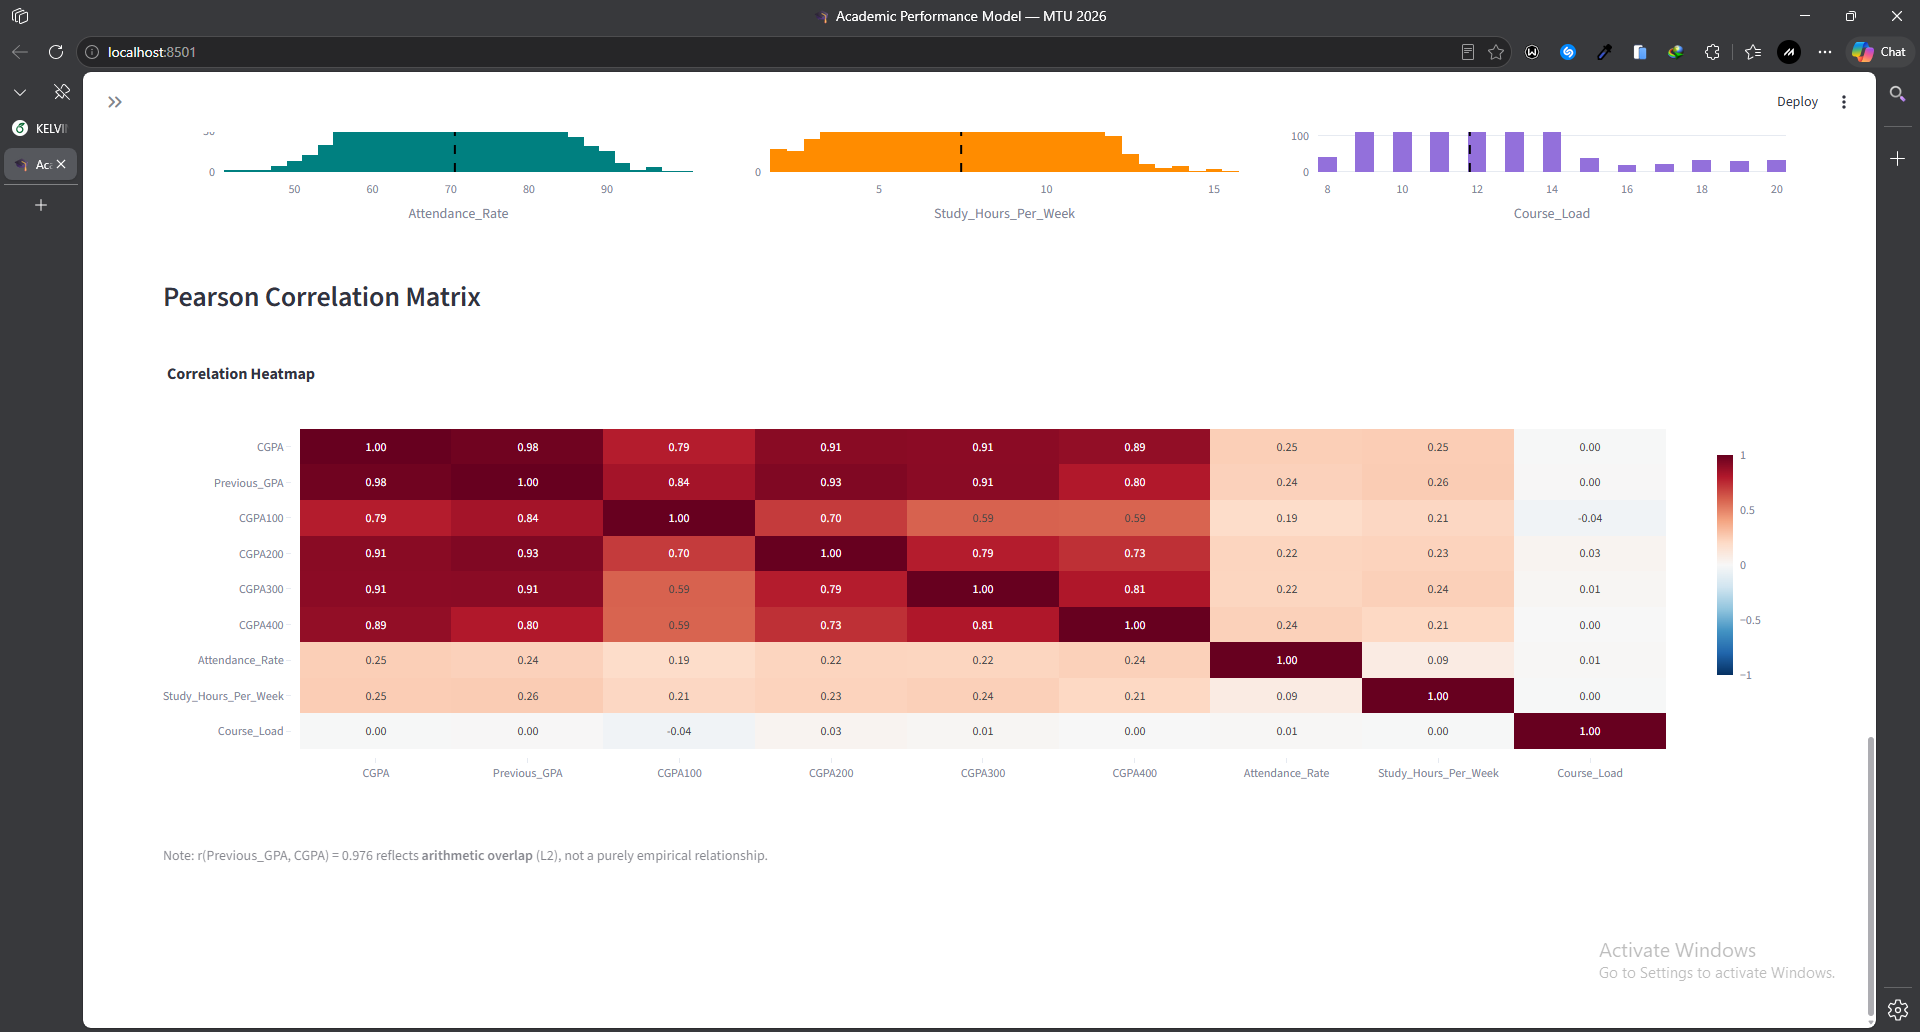
\includegraphics[width=0.95\textwidth]{fig-4-2-correlation-heatmap.png}
		\caption{Pearson correlation heatmap (deduplicated sample). Note $r(\text{Previous\_GPA}, \text{CGPA}) \approx 0.98$ (L2); primary OLS uses CGPA400 as the dependent variable. Synthesized predictors (L3) show weak bivariate association with GPA columns.}
		\label{fig:correlation-heatmap}
	\end{figure}
	
	Despite this marginal bivariate correlation, \textit{Study\_Hours\_Per\_Week}
	was not significant in the full OLS model ($\hat{\beta}_4 \approx -0.0003$,
	$p = 0.939$), consistent with prior GPA and trajectory terms absorbing
	most explainable variance once conditioning is applied.
	
	\section{Regression Results}
	Table~\ref{tab:regression} reports OLS coefficients for Equation~(\ref{eq:full-model}). Adjusted $R^2 = 0.682$. \textit{Previous\_GPA} has $\hat{\beta}_1 \approx 0.851$ ($p < 0.001$): a one-point higher three-year mean is associated with approximately a 0.85-point higher CGPA400, holding other predictors fixed. \textit{Trajectory\_Slope\_Prior} has $\hat{\beta}_2 \approx 0.448$ ($p < 0.001$): a one GPA-point-per-level steeper prior trend is associated with approximately a 0.45-point higher CGPA400. \textit{Attendance\_Rate} remains positive and significant ($\hat{\beta}_3 \approx 0.005$, $p < 0.001$) but with a smaller marginal role once trajectory is included. Study hours, course load, genotype dummies, and the SS$\times$attendance interaction are not significant at $\alpha = 0.05$ ($n_{\text{SS}} = 37$).
	
	Figure~\ref{fig:ols-results} reproduces the Streamlit OLS tab for CGPA400 (re-capture after refit if coefficient table predates \textit{Trajectory\_Slope\_Prior}). \textit{Previous\_GPA}, \textit{Trajectory\_Slope\_Prior}, and \textit{Attendance\_Rate} are significant at $\alpha = 0.05$; genotype terms are not (L3, L7). Coefficients on synthesized behavioural variables must not be read as causal effects (L1).
	
	\begin{figure}[htbp]
		\centering
		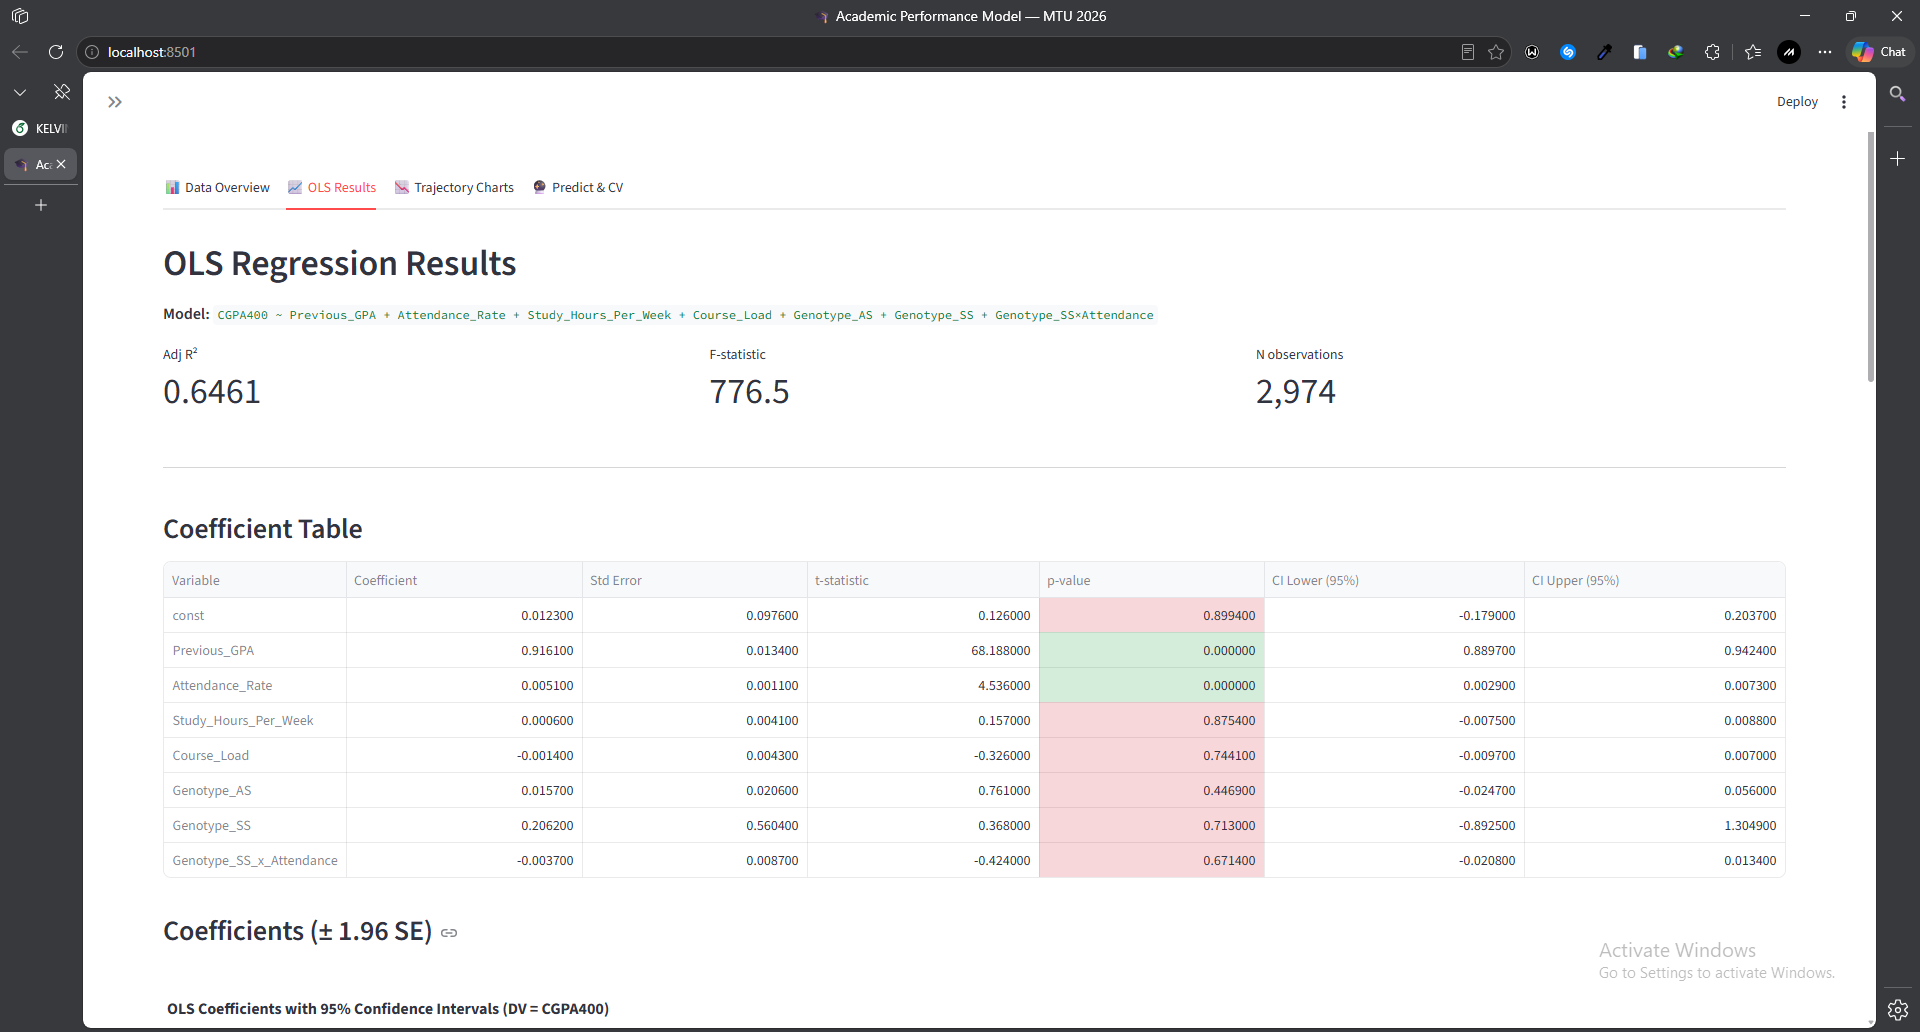
\includegraphics[width=0.92\textwidth]{fig-4-3-ols-results.png}
		\caption{OLS regression of CGPA400 ($n = 2{,}974$; adjusted $R^2 \approx 0.68$ after adding \textit{Trajectory\_Slope\_Prior}). Green cells: $p < 0.05$. Re-export from Streamlit if the table predates the trajectory predictor. Results are illustrative (L1).}
		\label{fig:ols-results}
	\end{figure}
	
	\begin{table}[htbp]
		\centering
		\caption{OLS regression of CGPA400 on predictors ($n = 2{,}974$; adjusted $R^2 = 0.682$)}
		\label{tab:regression}
		\begin{tabular}{lrrr}
			\hline
			Predictor & Coefficient & $p$-value & VIF \\
			\hline
			Previous\_GPA & 0.851 & $< 0.001$ & 1.22 \\
			Trajectory\_Slope\_Prior & 0.448 & $< 0.001$ & 1.10 \\
			Attendance\_Rate & 0.005 & $< 0.001$ & 1.10 \\
			Study\_Hours\_Per\_Week & $-0.0003$ & 0.939 & 1.07 \\
			Course\_Load & $-0.006$ & 0.166 & 1.01 \\
			Genotype (AS vs AA) & 0.009 & 0.658 & 1.02 \\
			Genotype (SS vs AA) & 0.186 & 0.726 & $\approx 50$* \\
			SS $\times$ Attendance & $-0.004$ & 0.615 & $\approx 50$* \\
			\hline
			\multicolumn{4}{l}{\footnotesize *Inflated VIF expected for SS block with interaction; main-effect VIF $< 10$.}
		\end{tabular}
	\end{table}
	
	\section{Model Diagnostics}
	Residual plots (residuals versus fitted values, normal Q--Q, histogram, and scale-location) are produced in \texttt{model.ipynb} and the Streamlit OLS tab. Residuals are more dispersed than in legacy CGPA models because CGPA400 is not arithmetically nested in \textit{Previous\_GPA}. Main-effect VIF values were below 10; the SS genotype block showed expected inflation.
	
	Figure~\ref{fig:residual-diagnostics} summarizes the four standard diagnostic panels. Residuals are approximately centred on zero with no strong funnel pattern; the Q--Q plot follows the normal reference line with minor tail deviation. The dashboard note applies: residual shape still reflects synthesis (L1--L3) and the strong \textit{Previous\_GPA} $\rightarrow$ CGPA400 relationship; diagnostics support use of OLS as an illustrative linear approximation, not proof of causal mechanisms.
	
	\begin{figure}[htbp]
		\centering
		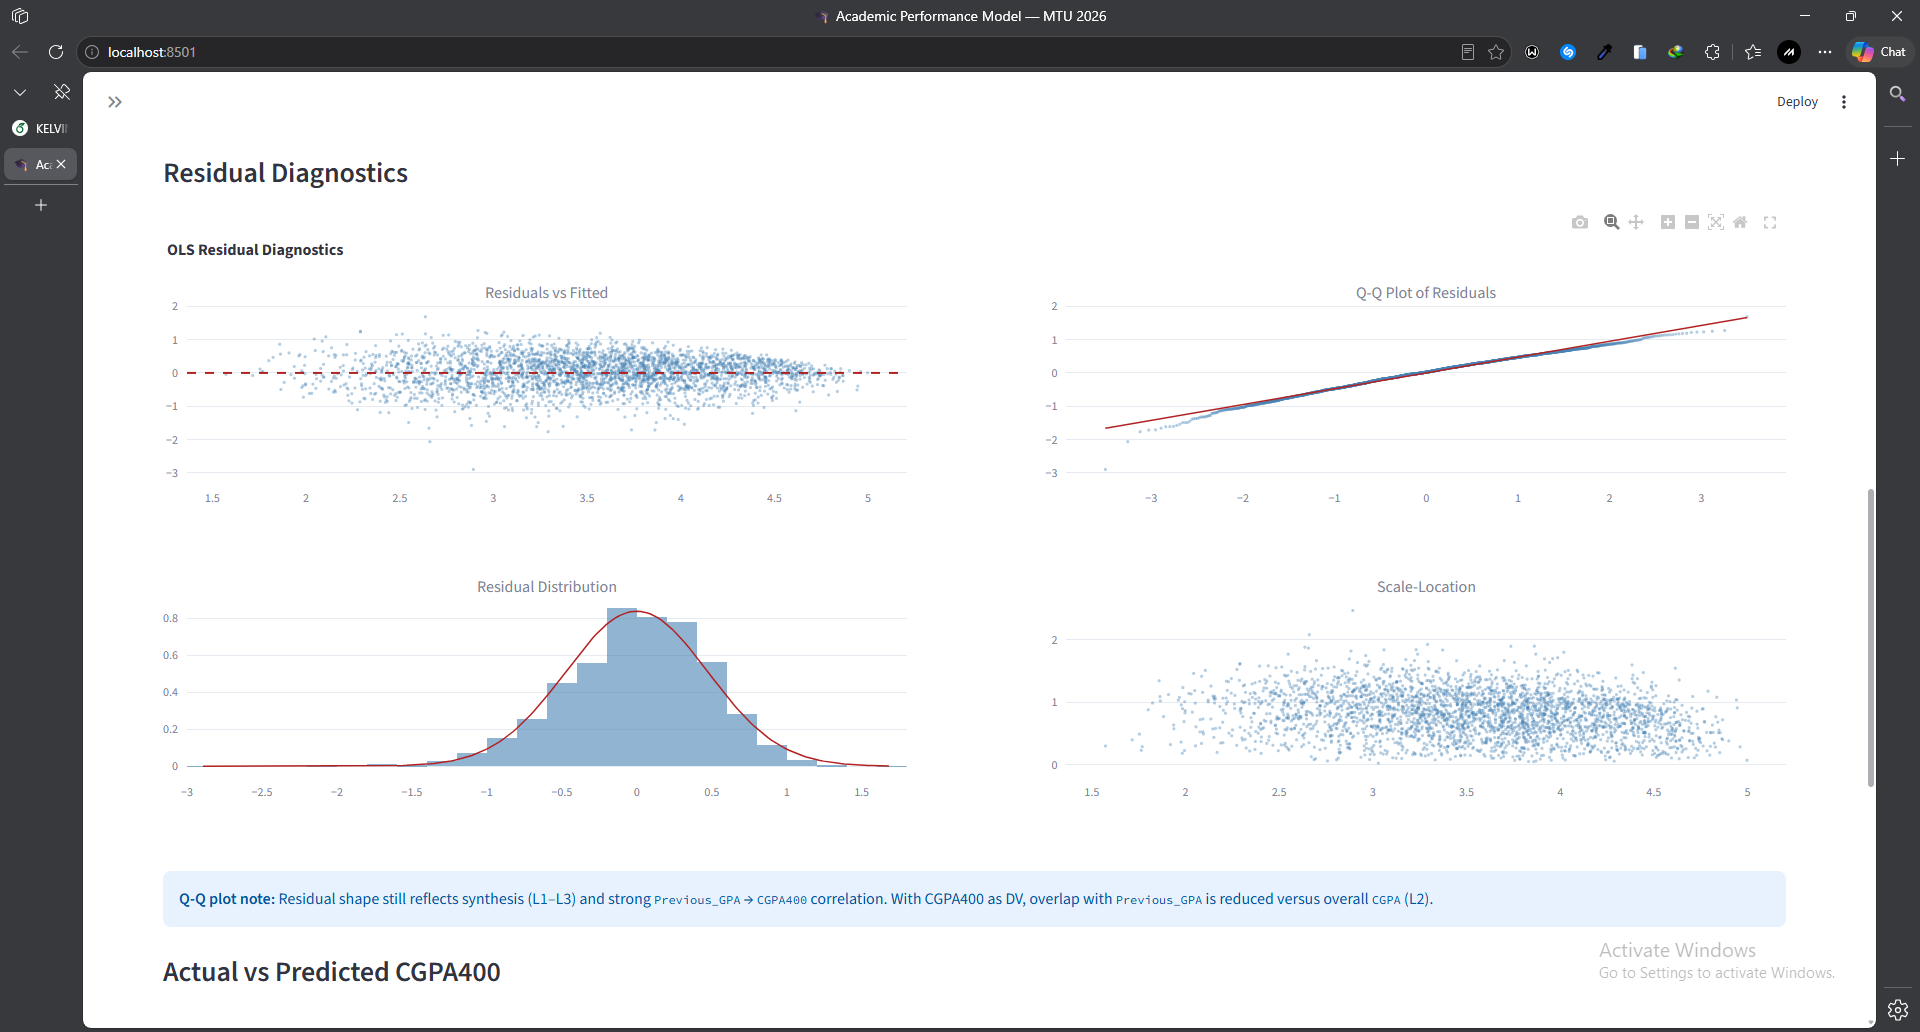
\includegraphics[width=0.95\textwidth]{fig-4-4-residual-diagnostics.png}
		\caption{Residual diagnostics for the CGPA400 OLS model. Panels: residuals versus fitted, Q--Q plot, residual histogram, and scale-location. Synthesis and lagged-GPA structure affect residual shape (L1, L2).}
		\label{fig:residual-diagnostics}
	\end{figure}
	
	\section{In-Sample Fit}
	The actual-versus-predicted CGPA400 scatter shows moderate scatter around the identity line (Adj $R^2 \approx 0.68$). This is a more honest fit than overall-CGPA models ($R^2 \approx 0.95$) and should not be cited as proof that attendance or genotype cause Level~400 outcomes (L1, L3, L7).
	
	Figure~\ref{fig:actual-vs-predicted} plots observed CGPA400 against in-sample fitted values, coloured by programme. Points cluster around the identity line for mid-range GPAs with greater dispersion at the lower end. Fit quality is dominated by \textit{Previous\_GPA} and \textit{Trajectory\_Slope\_Prior}; programme colour indicates heterogeneity across departments, not separate programme-specific models.
	
	\begin{figure}[htbp]
		\centering
		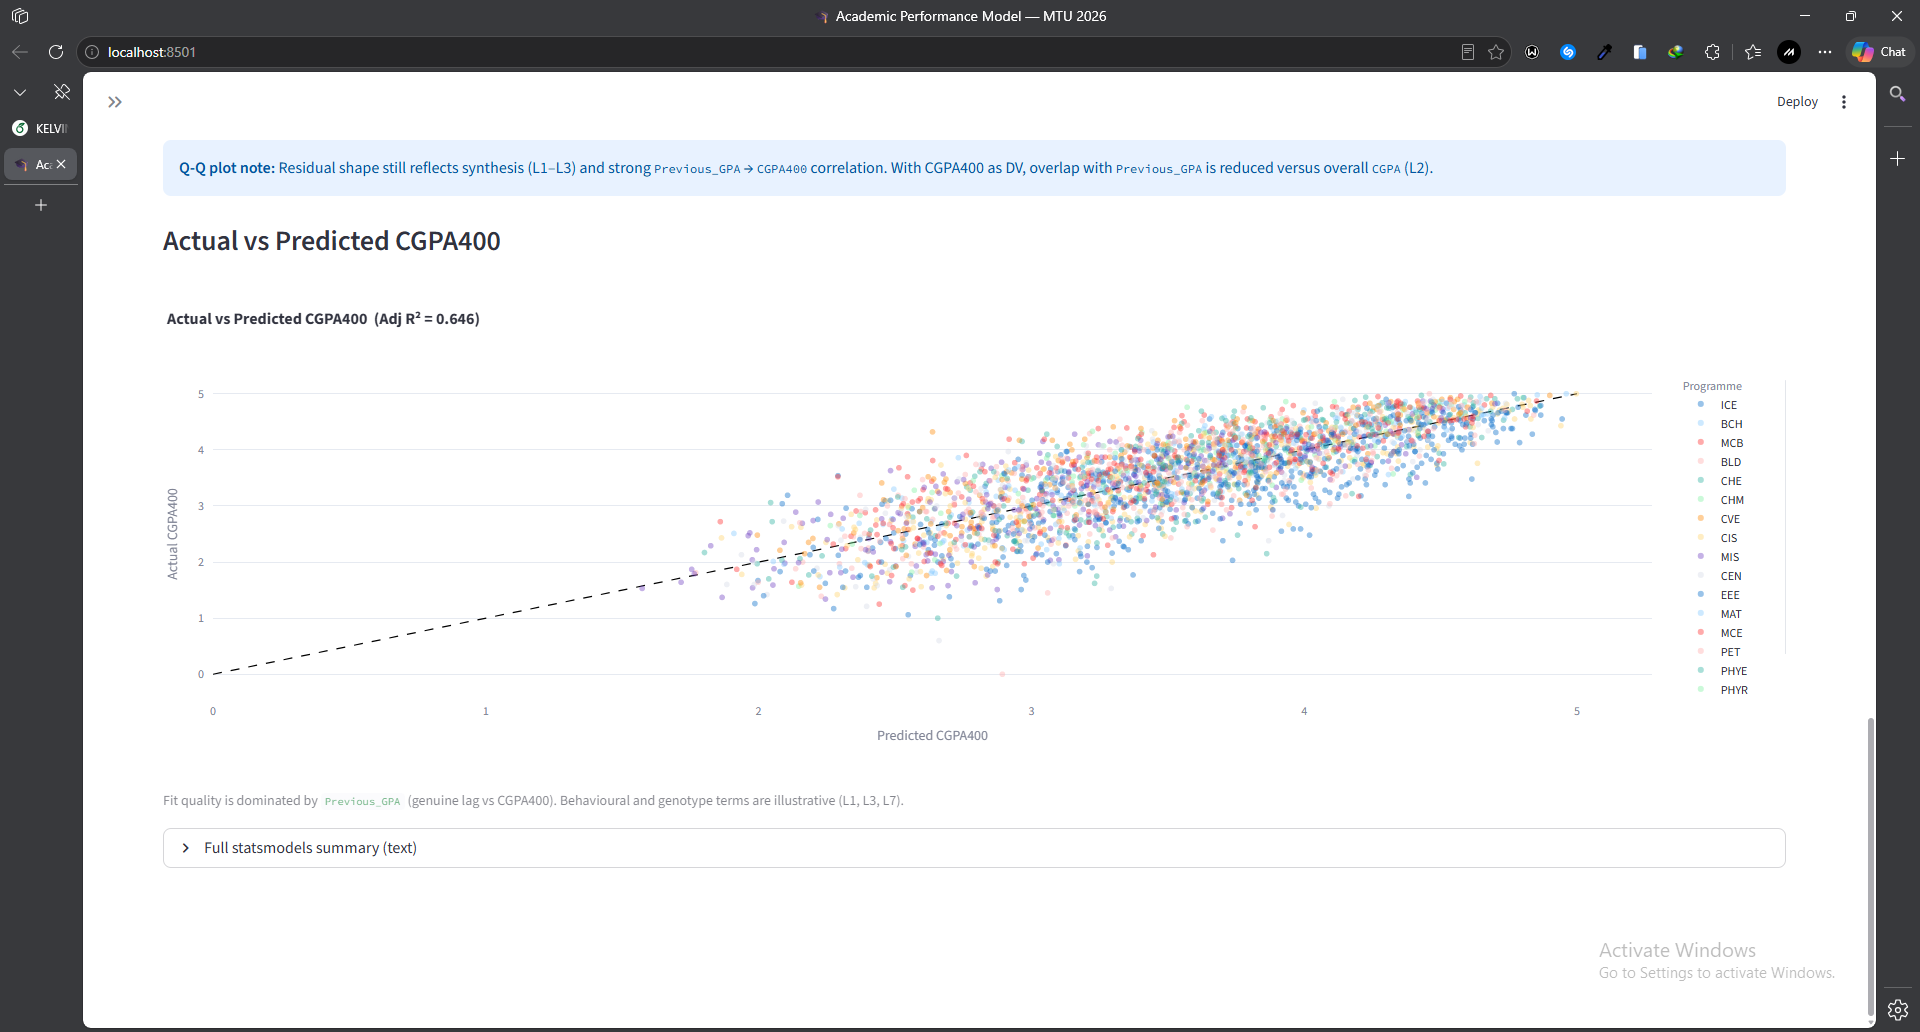
\includegraphics[width=0.92\textwidth]{fig-4-5-actual-vs-predicted.png}
		\caption{Actual versus predicted CGPA400 (adjusted $R^2 \approx 0.682$). Points coloured by programme code. Illustrative in-sample fit (L1); not a causal validation of behavioural or genotype predictors.}
		\label{fig:actual-vs-predicted}
	\end{figure}
	
	\section{Out-of-Sample Predictive Performance}
	Five-fold cross-validation (seed 42) yielded stacked out-of-fold MAE $= 0.357$, RMSE $= 0.453$, and $R^2 = 0.680$. The mean-only baseline achieved MAE $= 0.652$ and RMSE $= 0.802$. These metrics support the secondary predictive objective under the stated synthesis assumptions; they do not validate causal claims. The same metrics are reported interactively in the Streamlit \emph{Predict \& CV} tab (\texttt{streamlit run app.py}); a screenshot may be added to Appendix~A when captured.
	
	\section{Time-Series Analysis of Per-Level GPA}
	Using observed CGPA100--CGPA400, mean GPA trajectories were computed by programme and graduation year. Per-student \textit{Trajectory\_Slope} and \textit{Trajectory\_Class} (Improving / Stable / Declining) classify 1,168, 564, and 1,242 students respectively at a $\pm 0.05$ slope threshold. An AR(1) panel model on stacked level transitions ($\text{GPA}_t \sim \text{GPA}_{t-1}$) yielded $\hat{\phi}_1 = 0.773$ ($R^2 = 0.553$), quantifying academic momentum. Kendall's $\tau$ on the four-point cohort mean series was $\tau = 0$ ($p = 1.0$), indicating no monotonic cohort trend across levels in this cross-section.
	
	Figure~\ref{fig:trajectory-heatmap} shows mean GPA by programme and academic level (sorted by Level~400 performance). Each student contributes one observation per level; cell values are cohort means at each level, not repeated measurements of the same intake tracked over calendar time. Supplementary trajectory line charts and boxplots appear in Figure~\ref{fig:trajectory-composite} and Figure~\ref{fig:trajectory-by-programme} (Appendix~A).
	
	\begin{figure}[htbp]
		\centering
		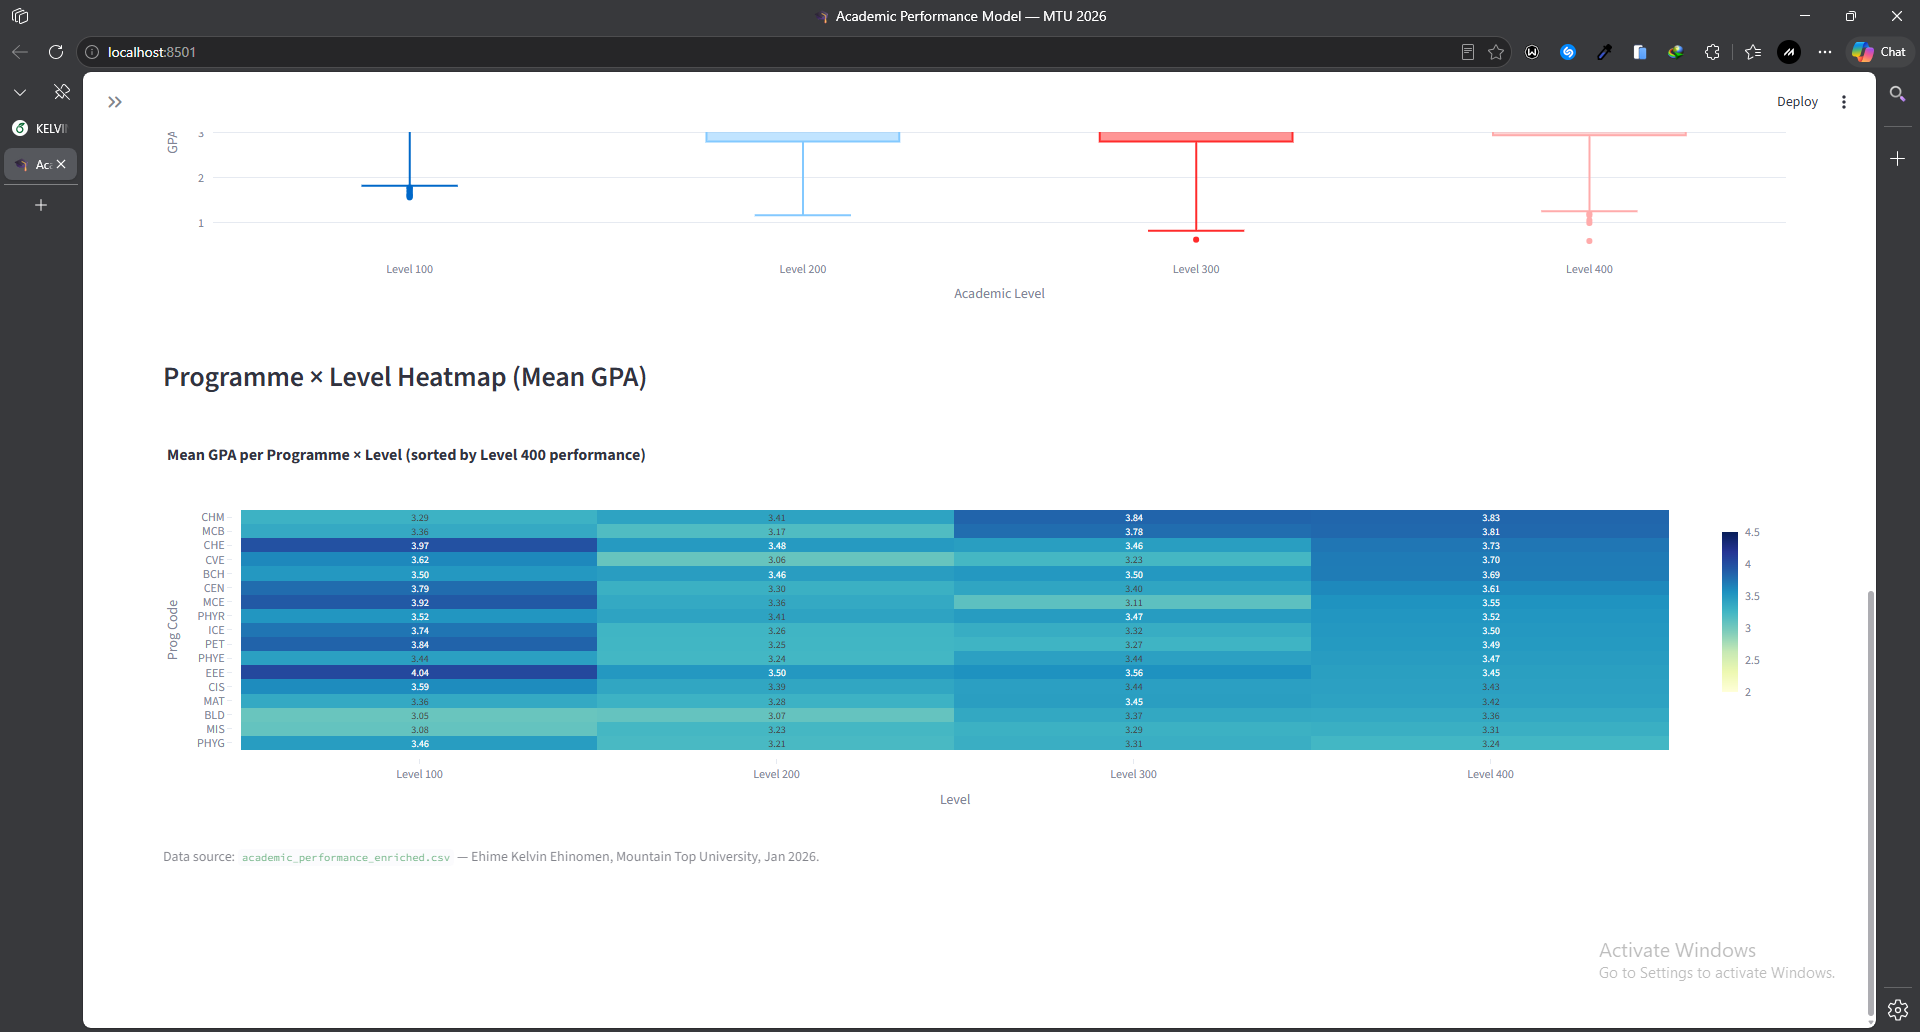
\includegraphics[width=0.95\textwidth]{fig-4-6-trajectory-heatmap.png}
		\caption{Programme $\times$ level heatmap of mean GPA (observed CGPA100--CGPA400). Rows sorted by Level~400 mean. Cross-sectional level progression: means across students at each level, not a single cohort followed over calendar years.}
		\label{fig:trajectory-heatmap}
	\end{figure}
	
	\section{Predictive Use Case}
	The scoring utility accepts new rows with the predictors in Table~\ref{tab:data-sources} and returns \texttt{predicted\_CGPA400}. The Streamlit \emph{Predict \& CV} tab exposes the same logic interactively (see Section~\ref{sec:oof-cv-note} in Appendix~A).
	
	\section{Summary of Findings}
	\begin{itemize}
		\item Prior three-year academic performance (\textit{Previous\_GPA}) is the dominant linear predictor of CGPA400.
		\item Reframing the DV to CGPA400 lowers adjusted $R^2$ from $\approx 0.95$ (CGPA) to $\approx 0.68$ with prior trajectory in the spec, a more honest range.
		\item \textit{Trajectory\_Slope\_Prior} and \textit{Previous\_GPA} are the dominant predictors; synthesized attendance remains significant but secondary.
		\item Out-of-sample MAE $\approx 0.36$ on a 5-point scale; AR(1) momentum $\hat{\phi}_1 \approx 0.77$.
		\item Per-level trajectory and classification analyses characterize observed GPA progression.
	\end{itemize}
	
	\section{Limitations of the Results}
	\label{sec:limitations-results}
	\textbf{L1 (Endogeneity):} Attendance and study hours retain CGPA-linked structure in synthesis; significant coefficients do not prove causal effects. \textbf{L2 (Overlap):} Primary DV is CGPA400 (no overlap with \textit{Previous\_GPA}); overall CGPA remains overlapping if used. \textbf{L3 (Synthesis):} Behavioural and load variables were not measured. \textbf{L4 (Overload):} 5\% overload rate is assumed. \textbf{L5 (IDs):} Duplicate ID collisions in source data. \textbf{L6 (Context):} MTU-specific calibration. \textbf{L7 (Genotype):} Genotype and attendance shifts are simulated, not clinically recorded. Results are illustrative for methodology demonstration and institutional discussion, not registrar-certified forecasting without observed predictors.
	
	\chapter{Conclusion}
	
	\section{Introduction}
	This chapter summarises the principal findings of the study, discusses their implications for institutional and methodological practice, acknowledges the limitations under which the results must be interpreted, and presents recommendations for future research. It draws together the regression, predictive validation, and time series analyses presented in Chapters~3 and~4 into a coherent closing account of what was achieved and what remains to be done.
	
	\section{Summary of Findings}
	Prior academic performance (\textit{Previous\_GPA}, the mean of Level~100--300 GPAs) and prior trajectory (\textit{Trajectory\_Slope\_Prior}, the OLS slope through CGPA100--300) were the dominant linear predictors of Level~400 GPA (CGPA400), with $\hat{\beta}_1 = 0.851$ and $\hat{\beta}_2 = 0.448$ ($p < 0.001$ for both). Together they align the regression scorer with the time-series narrative: level and trend before final year, without using CGPA400 in the trajectory predictor.
	
	\textit{Attendance\_Rate} remained statistically significant ($\hat{\beta}_3 = 0.005$, $p < 0.001$) but is secondary once trajectory is included. Study hours, course load, and genotype dummies were not significant at $\alpha = 0.05$, consistent with the weak synthesis signal and the small SS subsample ($n_{\text{SS}} = 37$ in the modelling sample).
	
	The decision to reframe the dependent variable from overall CGPA to CGPA400, and to add \textit{Trajectory\_Slope\_Prior}, yielded adjusted $R^2 = 0.682$ (versus $\approx 0.95$ for overlapping CGPA models). Five-fold cross-validation yielded out-of-fold MAE $= 0.357$ and RMSE $= 0.453$ on a 0--5 scale, representing a 45\% reduction in mean absolute error relative to the naive baseline (MAE $= 0.652$). This is an honest and reproducible predictive result.
	
	The AR(1) panel model fitted on stacked level-GPA transitions ($n = 8{,}922$ observations from 2,974 students) yielded an autoregressive coefficient $\hat{\phi}_1 = 0.773$ ($p < 0.001$, $R^2 = 0.553$). This quantifies academic momentum: a student performing one GPA point above the cohort mean in a given level is expected to perform approximately 0.77 points above the mean in the following level. The Mann-Kendall test on the cohort-mean level series found no monotonic trend ($\tau = 0$, $p = 1.0$), consistent with the observed non-linear pattern---a dip at Level~200 (mean GPA $= 3.322$) relative to Level~100 ($3.635$), followed by recovery at Level~300 ($3.421$) and Level~400 ($3.533$). Trajectory classification identified 1,168 improving students (39.3\%), 1,242 declining students (41.8\%), and 564 stable students (19.0\%) at a $\pm 0.05$ slope threshold.
	
	The health-pathway genotype inclusion---in which SS students were assigned a mean attendance penalty of 7.7 percentage points relative to AA students under the synthesis assumptions---produced the expected directional pattern in the data. The SS $\times$ Attendance interaction term ($\hat{\beta}_8 = -0.004$, $p = 0.615$) was not significant, which is attributed to the small SS subsample rather than absence of the pathway. This result is illustrative and consistent with the stated design intent; it does not constitute clinical evidence of a genotype effect on academic performance.
	
	\section{Implications of the Study}
	The dominance of \textit{Previous\_GPA} as a predictor suggests that early identification of students with declining Level~100--200 trajectories could enable timely intervention before Level~400. The AR(1) coefficient of 0.773 means that academic underperformance is persistent but not deterministic: there is meaningful variance left unexplained, giving intervention programmes room to operate.
	
	The study demonstrates the importance of choosing a dependent variable carefully. Using overall CGPA inflated $R^2$ to approximately 0.95 due to arithmetic overlap; switching to CGPA400 produced a more honest model that better represents a genuine prediction problem. Future studies in similar settings should attend to this distinction.
	
	By combining regression analysis with time series methods (AR(1), trajectory slopes, and the Mann-Kendall trend test on cohort means) in a single reproducible pipeline (\texttt{enrich.py}, \texttt{verify.py}, \texttt{model.ipynb}, \texttt{app.py}), the study provides a more complete characterisation of academic performance dynamics than either method alone would permit. Chapter~4 figures were exported from the Streamlit dashboard after running \texttt{streamlit run app.py} on the verified enriched dataset.
	
	\section{Limitations of the Study}
	\textbf{L1 --- Residual endogeneity.} Attendance and study hours were synthesized with a 40\% CGPA-linked component. Although the blended design reduces tautological regression, the significant attendance coefficient cannot be interpreted as causal evidence. Observed attendance records from the institution's registry would be required to make a causal claim.
	
	\textbf{L2 --- Previous\_GPA and CGPA overlap (resolved for primary DV).} The primary dependent variable CGPA400 has no arithmetic overlap with \textit{Previous\_GPA}. However, if overall CGPA were used as the DV, the overlap would return and inflate $R^2$ artificially, as demonstrated by the legacy comparison ($R^2 \approx 0.95$). Researchers adopting similar designs should be alert to this distinction.
	
	\textbf{L3 --- Synthesized behavioural variables.} \textit{Attendance\_Rate}, \textit{Study\_Hours\_Per\_Week}, and \textit{Course\_Load} were not recorded in the source dataset and were generated under documented statistical assumptions. The enriched dataset should be treated as a methodology demonstration, not as a record of actual student behaviour.
	
	\textbf{L4 --- Overload rate assumption.} Approximately 5\% of students were assigned an approved course overload (16--20 courses) based on an assumed institutional rate, not a verified registrar figure. This affects \textit{Course\_Load} distributions for a small subset of students.
	
	\textbf{L5 --- Duplicate ID collisions.} The source dataset contained 72 duplicate \textit{ID No} entries across students with different programme codes, genders, or graduation years, indicating data-entry errors in the original registrar export. De-duplication retained the first occurrence ($n = 2{,}974$ for regression), but the underlying ID collision issue cannot be resolved without access to the original registrar system.
	
	\textbf{L6 --- Institutional specificity.} All synthesis parameters (programme load distributions, attendance means, genotype priors) were calibrated for Mountain Top University and the Nigerian population context. The model is not directly transferable to other institutions without re-calibration.
	
	\textbf{L7 --- Synthesized genotype and low SS power.} Haemoglobin genotype was not available in the registrar export and was assigned by multinomial draw. The health-pathway attendance shift for SS students is an assumed relationship grounded in the sickle cell literature, not a clinically verified one. With only 37 SS students in the modelling sample, the SS $\times$ Attendance interaction term has insufficient statistical power to detect a meaningful effect even if one exists. A study specifically designed to test this hypothesis would require a larger and clinically verified sample.
	
	\section{Recommendations for Future Research}
	\begin{enumerate}
		\item \textbf{Collect observed behavioural data.} The most direct improvement would be to replace synthesized attendance and study hours with observed records from the institution's learning management system or attendance registers. This would allow the regression coefficients to be interpreted as genuine behavioural associations rather than illustrative ones.
		
		\item \textbf{Expand the SS genotype sample.} The health-pathway genotype hypothesis could be properly tested with a dedicated dataset that includes clinical genotype records and sufficient SS representation (a minimum of 100--200 SS students is recommended for adequate power on the interaction term). Collaboration with the institution's health services would enable this.
		
		\item \textbf{Apply longitudinal time series methods.} The AR(1) analysis in this study used cross-sectional data---students were not tracked as a true cohort over calendar time. A longitudinal design following one or more intake cohorts from Level~100 through Level~400 would enable proper time series modelling with stationarity testing, seasonal decomposition, and cohort-level forecasting.
		
		\item \textbf{Extend to multi-institution datasets.} The current model is calibrated for Mountain Top University. Replicating the pipeline across multiple Nigerian universities---or universities in other contexts---would allow the generalisability of the findings to be assessed and the synthesis parameters to be grounded in cross-institutional data rather than a single-institution prior.
	\end{enumerate}
	
	\section{Concluding Remarks}
	This study set out to develop a mathematical and statistical model to analyse and predict student academic performance at Mountain Top University using integrated academic, behavioural, and health-related predictors. That aim was achieved through a reproducible pipeline combining OLS regression on CGPA400, $k$-fold cross-validation, AR(1) time series analysis on per-level GPA transitions, and per-student trajectory classification. The use of synthesized data where registrar records were incomplete is a limitation, but it was a deliberate methodological choice made transparent throughout Chapters~3--5. Quantitative modelling of this kind, when applied with appropriate caution about data provenance and dependent-variable design, can support evidence-informed educational planning and early identification of students who may benefit from institutional intervention.
	
	\appendix
	\chapter{Supplementary Streamlit Figures}
	\label{ch:appendix-figures}
	
	This appendix holds exploratory and supplementary views from the Streamlit dashboard (\texttt{streamlit run app.py}) that support Chapter~4 but are not required for the main narrative thread.
	
	\begin{figure}[htbp]
		\centering
		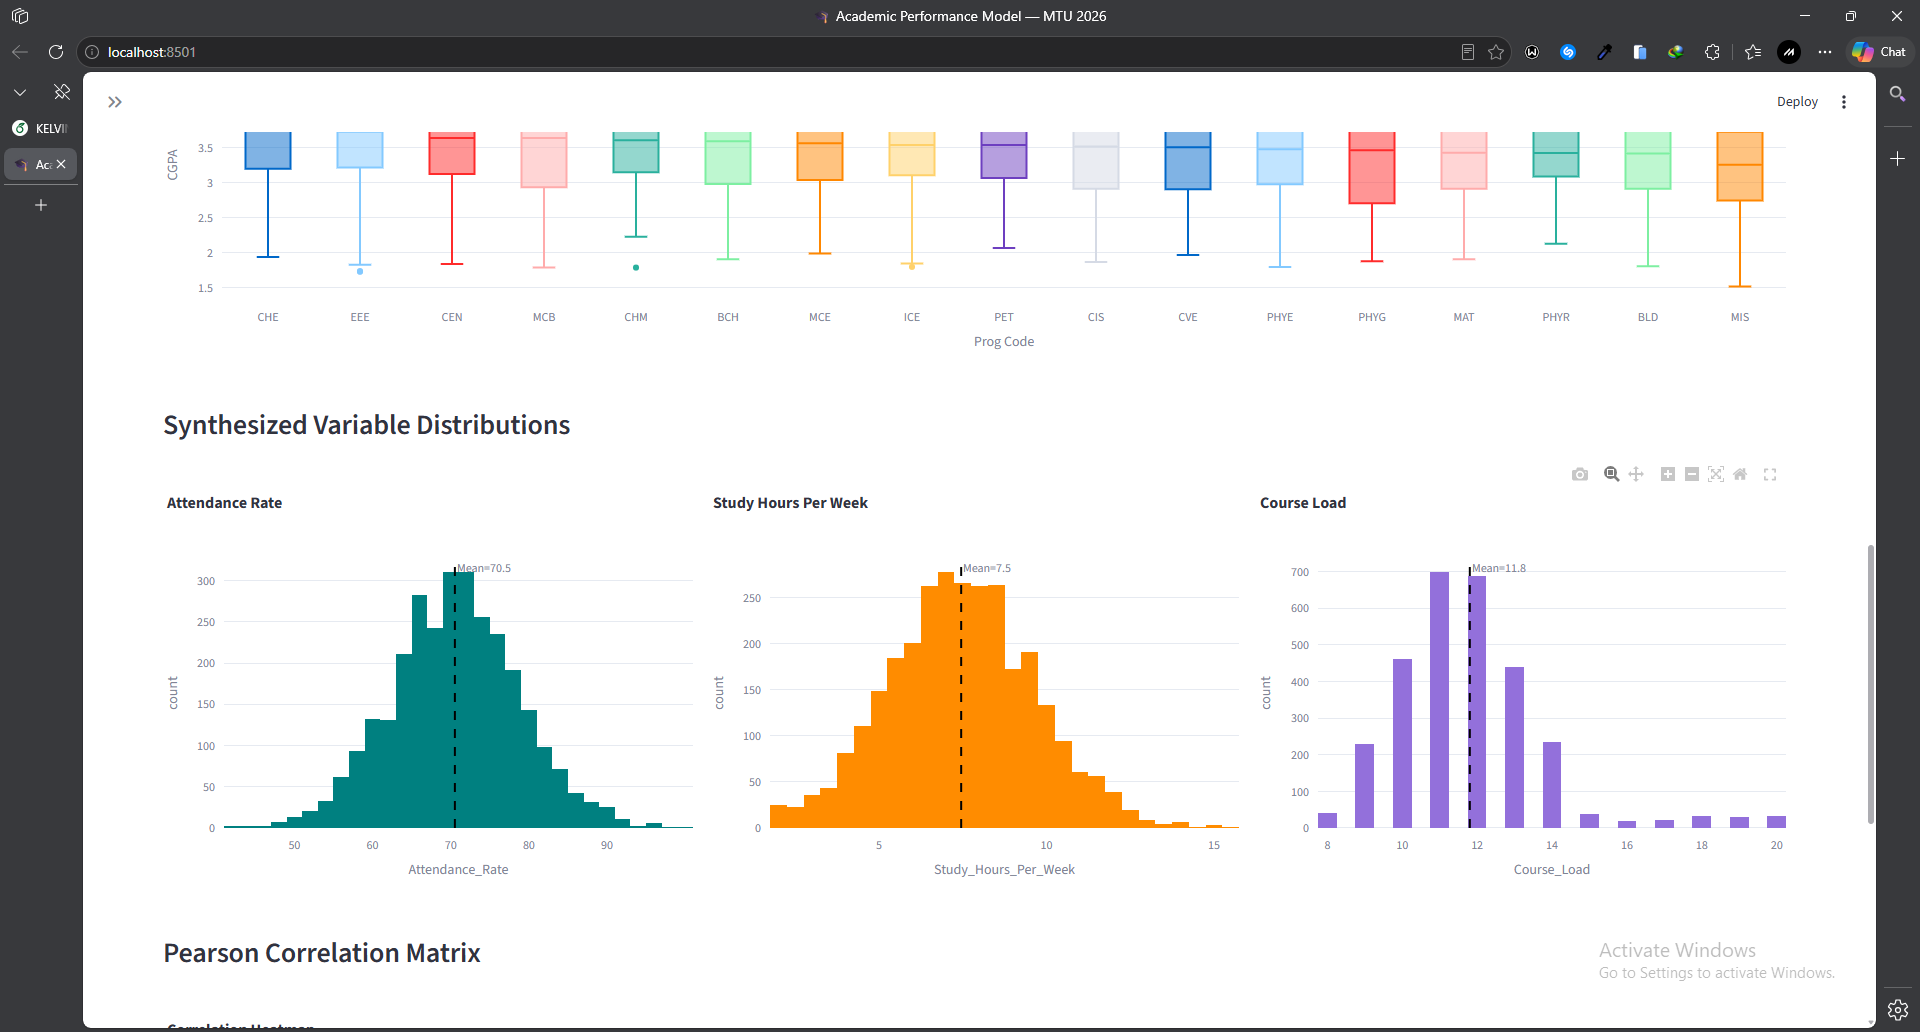
\includegraphics[width=0.92\textwidth]{fig-A-1-cgpa-distributions.png}
		\caption{CGPA distribution (histogram), CGPA by gender (violin plots), and synthesized variable histograms (attendance, study hours, course load).}
		\label{fig:appendix-distributions}
	\end{figure}
	
	\begin{figure}[htbp]
		\centering
		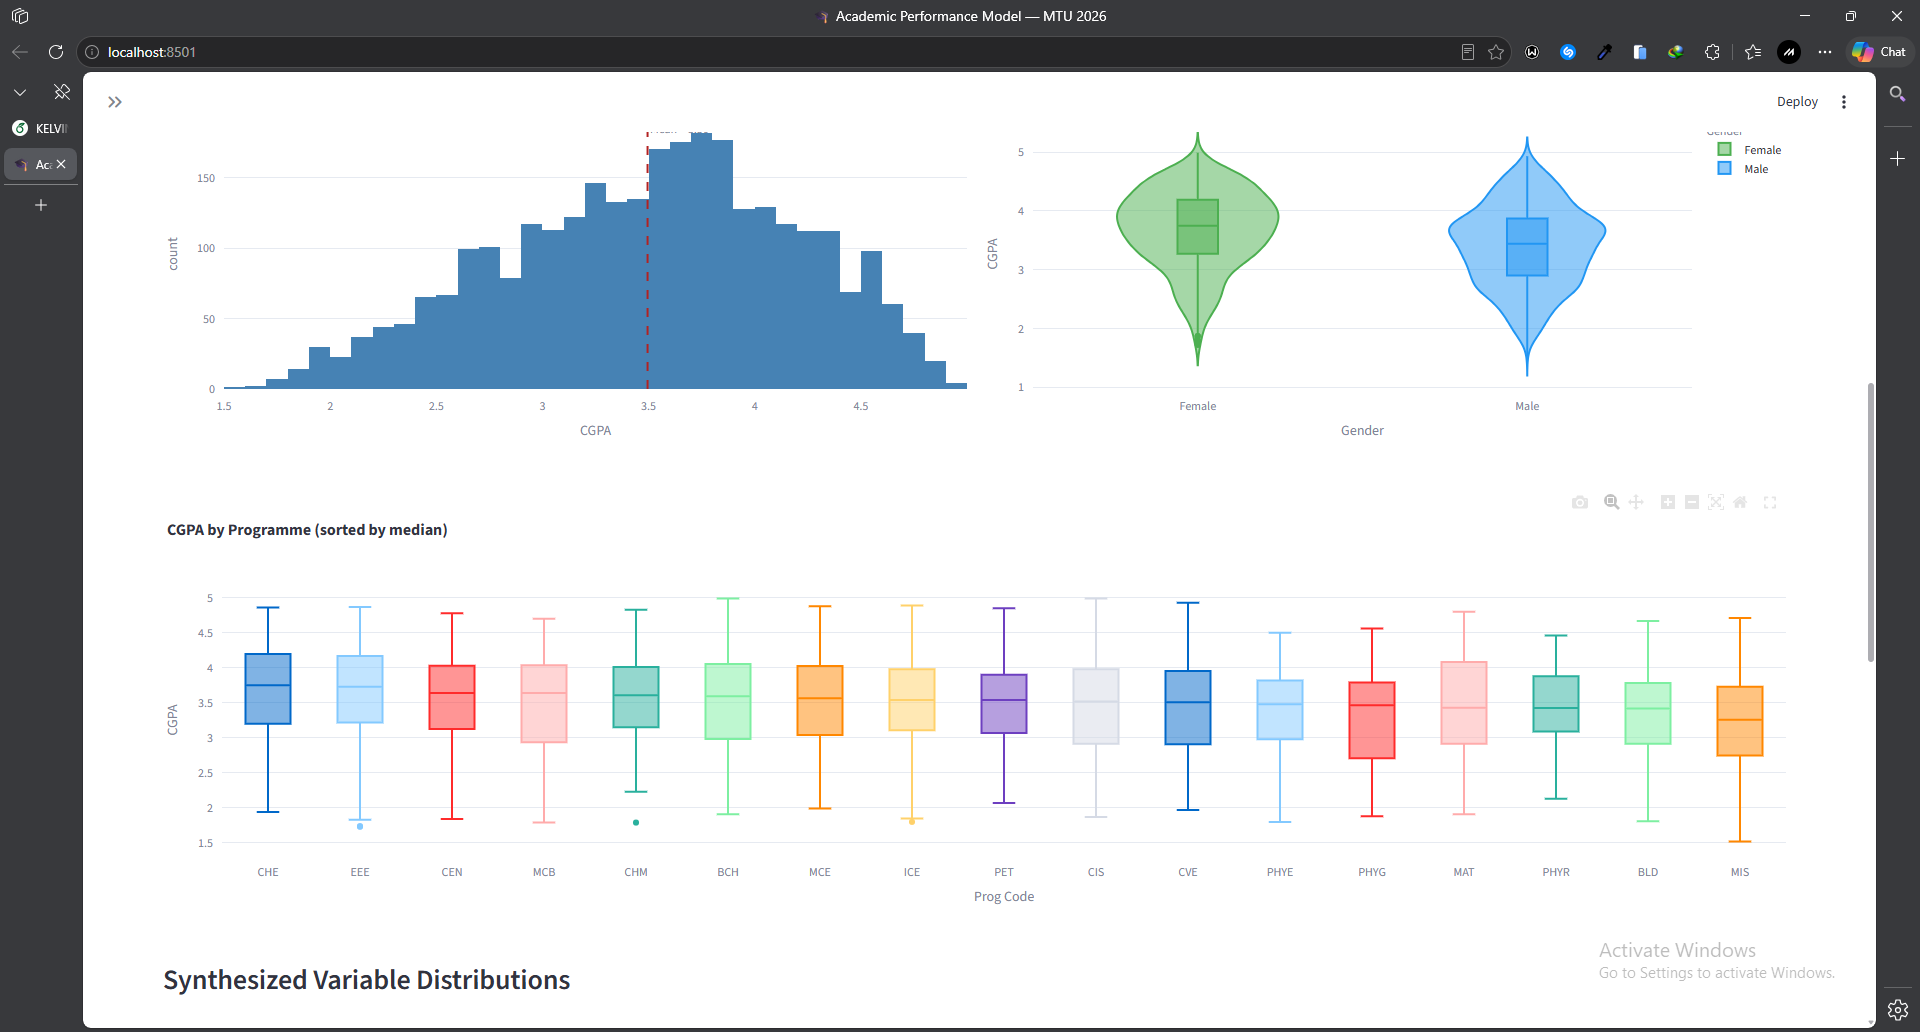
\includegraphics[width=0.92\textwidth]{fig-A-2-cgpa-by-gender-programme.png}
		\caption{CGPA distribution with mean marker, gender comparison, and programme box plots sorted by median CGPA.}
		\label{fig:appendix-gender-programme}
	\end{figure}
	
	\begin{figure}[htbp]
		\centering
		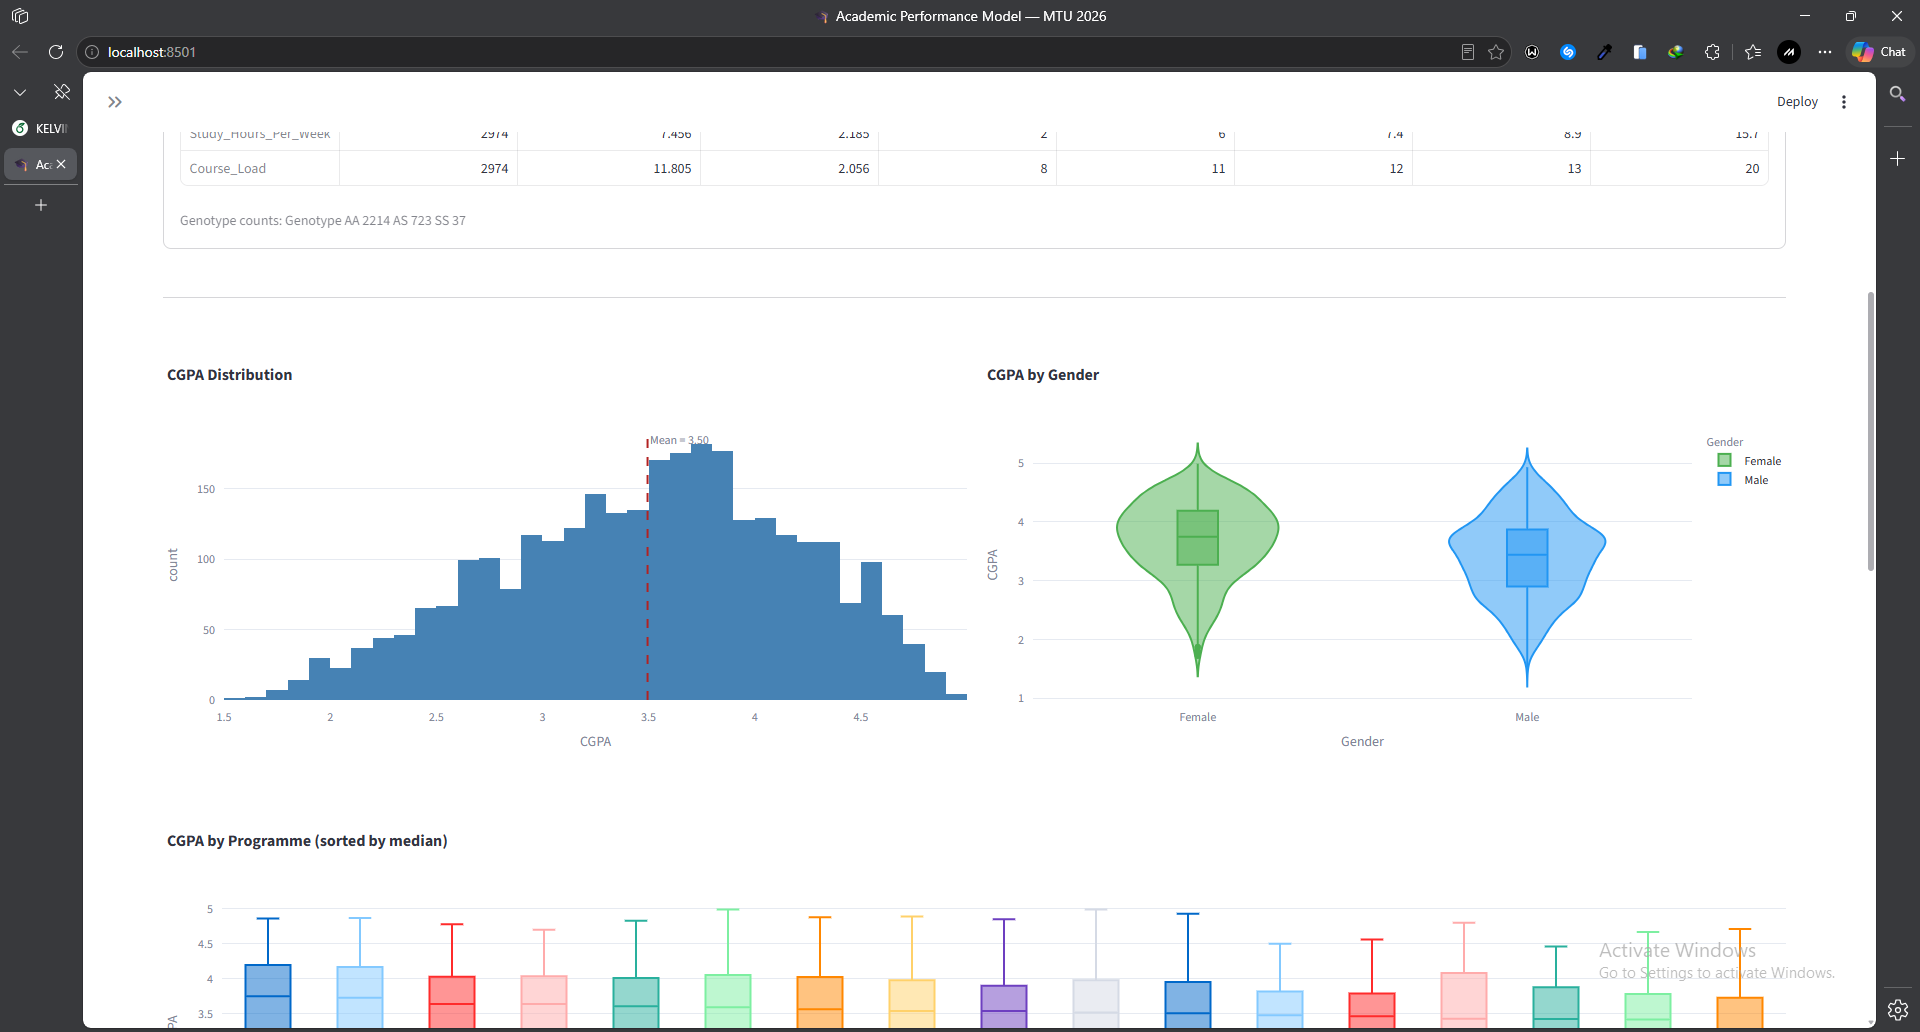
\includegraphics[width=0.92\textwidth]{fig-A-3-synthesized-histograms.png}
		\caption{Programme-level CGPA box plots and synthesized predictor distributions (L3).}
		\label{fig:appendix-synthesized}
	\end{figure}
	
	\begin{figure}[htbp]
		\centering
		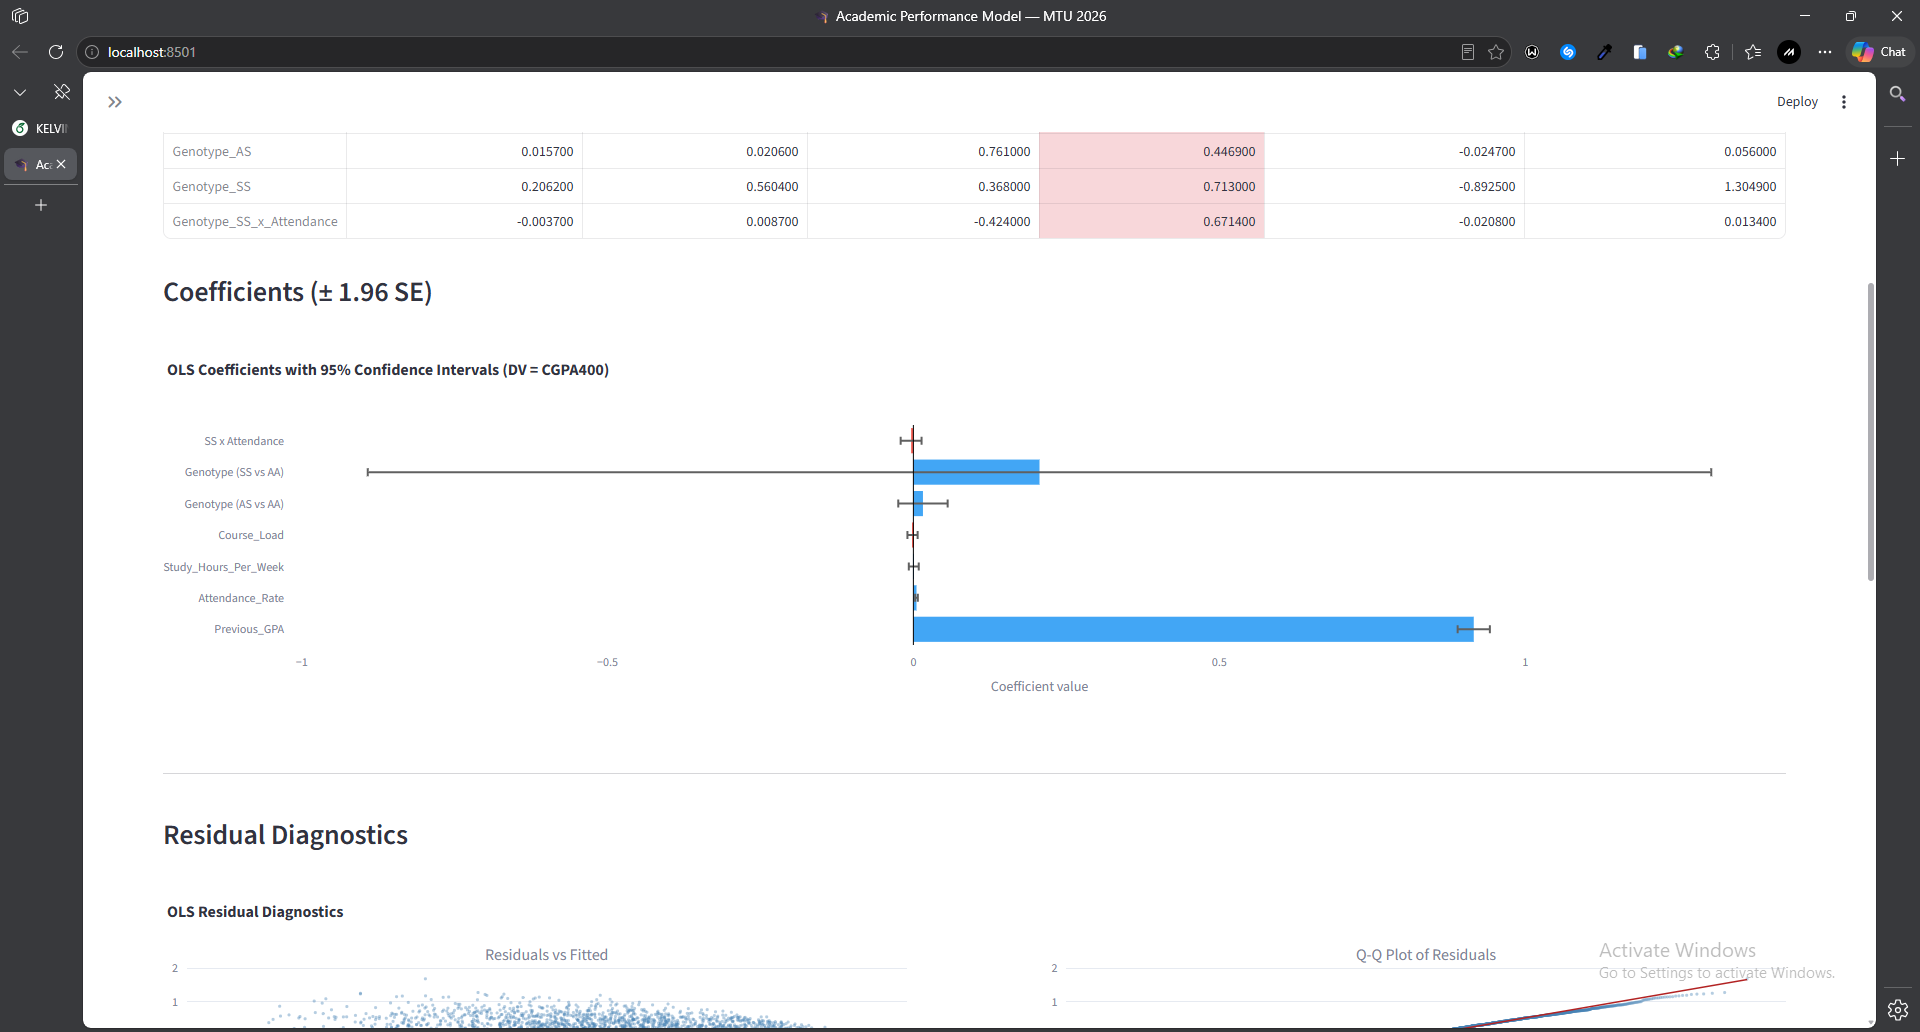
\includegraphics[width=0.92\textwidth]{fig-A-5-ols-coefficients-ci.png}
		\caption{OLS coefficients with 95\% confidence intervals (DV = CGPA400). Wide intervals for genotype SS reflect small $n_{\text{SS}}$ (L7).}
		\label{fig:appendix-ols-ci}
	\end{figure}
	
	\begin{figure}[htbp]
		\centering
		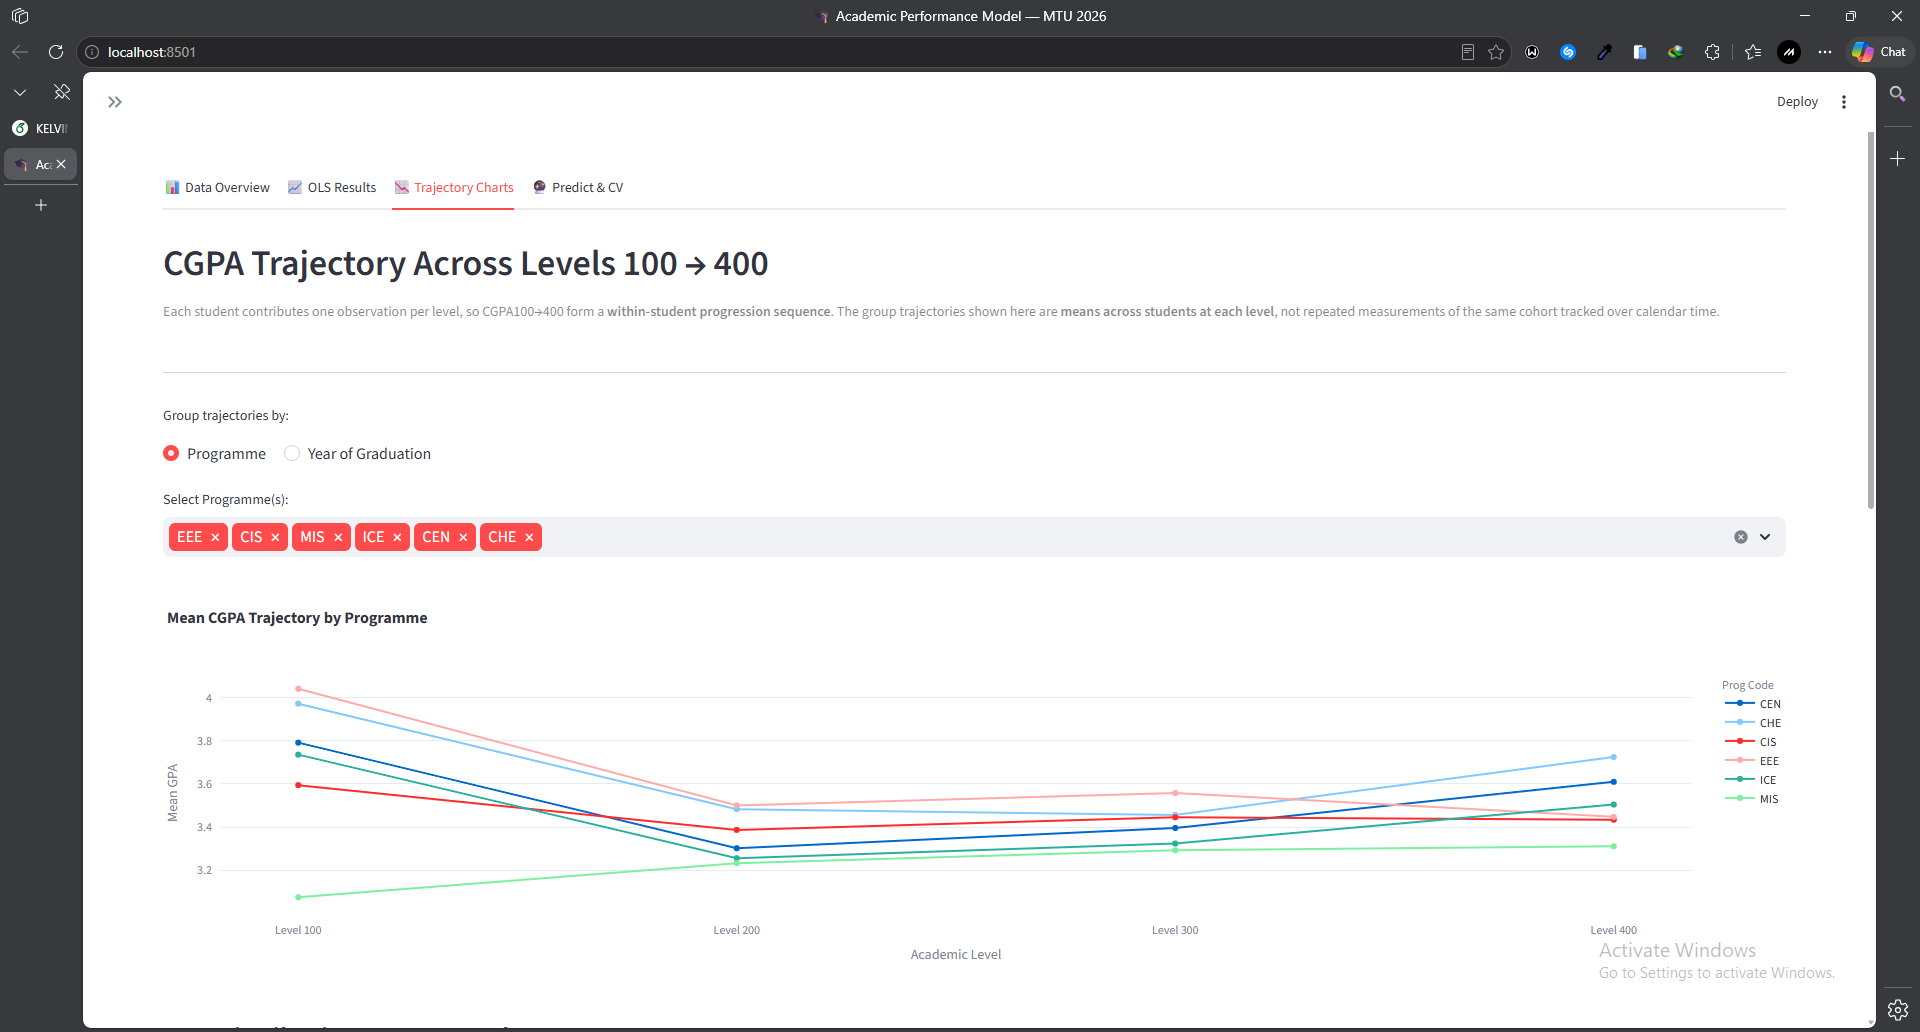
\includegraphics[width=0.95\textwidth]{fig-A-6-trajectory-by-programme.png}
		\caption{Mean CGPA trajectory by selected programmes (Level~100--400). Each line is the mean across students at each level, not calendar-year cohort tracking.}
		\label{fig:trajectory-by-programme}
	\end{figure}
	
	\begin{figure}[htbp]
		\centering
		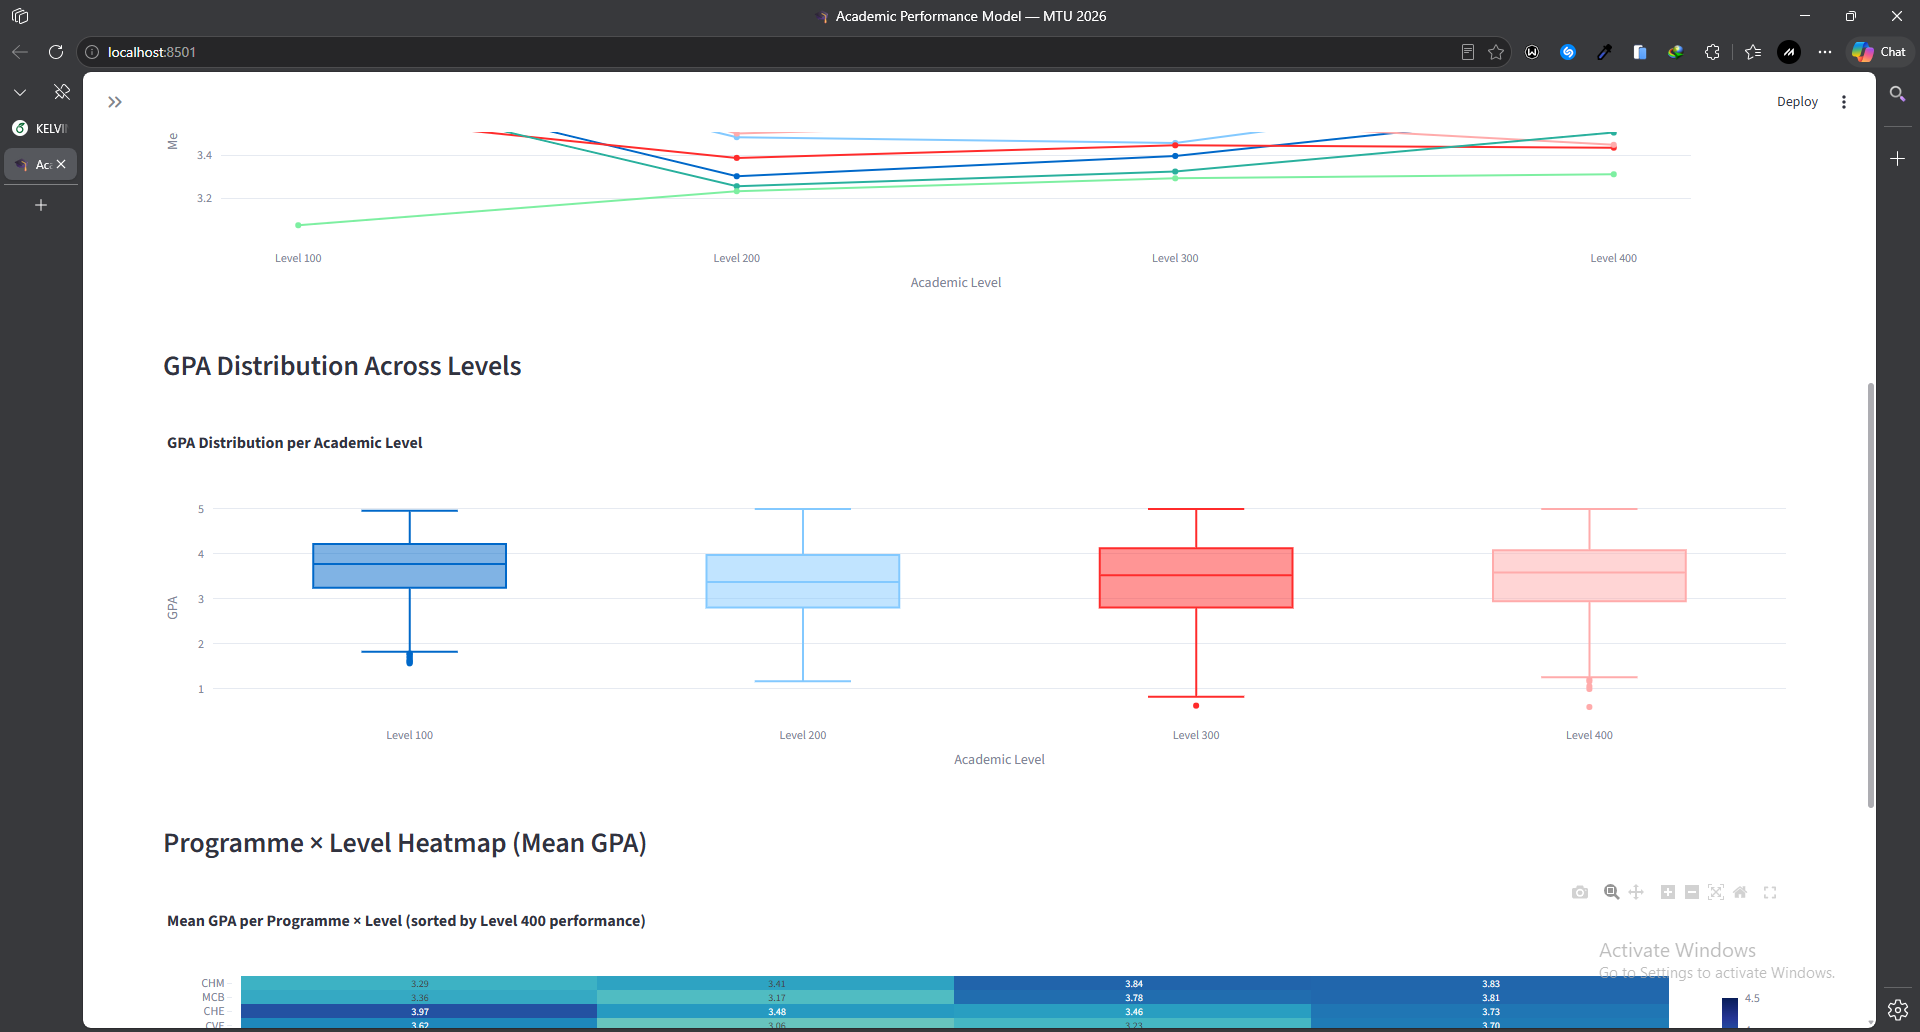
\includegraphics[width=0.95\textwidth]{fig-A-4-trajectory-composite.png}
		\caption{Composite trajectory tab: mean lines by programme, GPA box plots by level, and programme $\times$ level heatmap.}
		\label{fig:trajectory-composite}
	\end{figure}
	
	\section{Out-of-Sample Metrics in the Dashboard}
	\label{sec:oof-cv-note}
	Five-fold cross-validation metrics (MAE $= 0.357$, RMSE $= 0.453$, out-of-fold $R^2 = 0.680$) are reported in text in Section~4.6 and interactively under the Streamlit \emph{Predict \& CV} tab. To include a figure, capture a screenshot after \texttt{streamlit run app.py} and add \texttt{fig-A-8-predict-cv.png} to \texttt{docs/PROJECT-MAIN/img/}.
	
	\newpage
	\bibliographystyle{plainnat}
	\bibliography{references}

\end{document}